\chapter{Results and Discussion}\label{ch5:chapter5}


\section{Experiments results Database }\label{ch5:database}

The main objective of this study was to propose an evaluation of three failure criteria for a selected rock, Dunnville Sandstone. As explained in the previous chapters, their empirical nature requires a thick database of diverse multi axial experiments for their development. 

Dunnville Sandstone have been used for several works in the past and particularly for multi axial experiments \cite{Labuz2018}\cite{Zeng2019}\cite{Tarokh2016}. The ones performed in the scope of this study (cf. Chapter \ref{ch4:title}) presented the opportunity to enrich the existing tests results database and to evaluate the failure criteria with data representative of Dunnville Sandstone response.

The database presented in Table \ref{tb5:database} was based on the one proposed by Zeng et al. (2019) \cite{Zeng2019}, and extended with the results of the experiments from this study. In this table, each experiment is associated with the following elements: the orientation of the bedding regarding the application of the axial stress, the three principal stresses (i.e. $\sigma_I$,$\sigma_{II}$,$\sigma_{III}$) and the stress invariants (i.e.$p$, $q$, $\theta$).

This database was used for the evaluation of Mohr-Coulomb,Hoek-Brown and Paul-Mohr-Coulomb failure criteria, that will be presented in the following sections.

\begin{table}
    \centering
    \begin{tabular}{cccccccc}
        \hline 
        Test & Bedding & $\sigma_I$ [\si{MPa}] & $\sigma_{II}$ [\si{MPa}] &$\sigma_{III}$ [\si{MPa}] & $p$ [\si{MPa}] & $q$ [\si{MPa}] & $\theta$ [\si{\degree}] \\
        \hline
        \hline
        Published TC-1 & \(\perp\) & 29.7 & 0.0 & 0.0 & 9.9 & 29.7 & 0 \\
        Published TC-2 & \(\perp\) & 39.4 & 2.5 & 2.5 & 14.8 & 36.9 & 0 \\
        Published TC-3 & \(\perp\) & 52.9 & 5.0 & 5.0 & 21.0 & 47.9 & 0 \\
        Published TC-4 & \(\perp\) & 71.5 & 10.0 & 10.0 & 30.5 & 61.5 & 0 \\
        Published TC-5 & \(\perp\) & 98.4 & 20.0 & 20.0 & 46.1 & 78.4 & 0 \\
        Published TC-6 & \(\perp\) & 114.5 & 30.0 & 30.0 & 58.2 & 84.5 & 0 \\
        Published TC-7 & \(\perp\)& 129.4 & 40.0 & 40.0 & 69.8 & 89.4 & 0 \\
        Published TC-8 & \(\perp\) & 142.1 & 50.0 & 50.0 & 80.7 & 92.1 & 0 \\
        Published TC-9 & \(\perp\) & 153.8 & 60.0 & 60.0 & 91.3 & 93.8 & 0 \\
        Published TC-10 & \(\|\) & 24.9 & 0.0 & 0.0 & 8.3 & 24.9 & 0 \\
        Published TC-11 & \(\|\) & 35.2 & 2.5 & 2.5 & 13.4 & 32.7 & 0 \\
        Published TC-12 & \(\|\) & 48.8 & 5.0 & 5.0 & 19.6 & 43.8 & 0 \\
        Published TC-13 & \(\|\) & 68.0 & 10.0 & 10.0 & 29.3 & 58.0 & 0 \\
        Published TC-14 & \(\|\) & 95.9 & 20.0 & 20.0 & 45.3 & 75.9 & 0 \\
        Published TC-15 & \(\|\) & 110.9 & 30.0 & 30.0 & 57.0 & 80.9 & 0 \\
        Published TC-16 & \(\|\) & 125.5 & 40.0 & 40.0 & 68.5 & 85.5 & 0 \\
        Published TC-17 & \(\|\) & 138.1 & 50.0 & 50.0 & 79.4 & 88.1 & 0 \\
        Published TC-18 & \(\|\) & 150.8 & 60.0 & 60.0 & 90.3 & 90.8 & 0 \\
        UCS   & \(\perp\) & 29.8 & 0 & 0   & 27.95 & 51.43 & 0 \\ 
        TC 9  & \(\perp\) & 49.43 & 5  & 5 & 19.81 & 44.43 & 0 \\ 
        TC 0  & \(\perp\) & 61.43 & 10 & 10 & 27.95 & 51.43 & 0 \\ 
        TC 5  & \(\perp\) & 91.08 & 20 & 20 & 44.72 & 71.08 & 0 \\ 
        TC 8  & \(\perp\) & 127.3 & 40 & 40 & 65.73 & 87.30 & 0 \\ 
        TC 10 & \(\perp\) & 151.1 & 60 & 60 & 88.12 & 91.10 & 0 \\ 
        \hline
        \hline
        Published TE-1 & \(\perp\) & 35.0 & 35.0 & 0.8 & 23.6 & 34.2 & 60 \\
        Published TE-2 & \(\perp\) & 40.0 & 40.0 & 1.2 & 27.1 & 38.8 & 60 \\
        Published TE-3 & \(\perp\) & 50.0 & 50.0 & 6.0 & 35.3 & 44.0 & 60 \\
        Published TE-4 & \(\perp\) & 60.0 & 60.0 & 10.1 & 43.4 & 49.9 & 60 \\
        Published TE-5 & \(\perp\) & 69.0 & 69.0 & 11.5 & 49.8 & 57.5 & 60 \\
        Published TE-6 & \(\|\) & 40.0 & 40.0 & 1.8 & 27.3 & 38.2 & 60 \\
        Published TE-7 & \(\|\) & 50.0 & 50.0 & 5.7 & 35.2 & 44.3 & 60 \\
        Published TE-8 & \(\|\) & 60.0 & 60.0 & 8.0 & 42.7 & 52.0 & 60 \\
        TE 3  & \(\perp\) & 35 & 35 & 3.96 & 24.64 & 31.08 & 60 \\ 
        TE 1  & \(\perp\) & 40 & 40 & 4.50 & 27.89 & 36.34 & 60 \\ 
        TE 2  & \(\perp\) & 60 & 60 & 9.68 & 43.01 & 50.98 & 60 \\
        \hline
        \hline
        Published TT-1 & \(\perp\) & 48.3 & 31.6 & 5.0 & 28.3 & 37.8 & 37.5 \\
        Published TT-2 & \(\perp\) & 52.9 & 25.1 & 7.0 & 28.3 & 40.1 & 22.7 \\
        Published TT-3 & \(\perp\) & 63.9 & 12.1 & 9.0 & 28.3 & 53.4 & 2.9 \\
        Published TT-4 & \(\perp\) & 70.6 & 49.4 & 15.0 & 45.0 & 48.7 & 37.8 \\
        Published TT-5 & \(\perp\) & 77.5 & 70.5 & 20.0 & 56.0 & 54.3 & 53.5 \\
        Published TT-6 & \(\perp\) & 83.9 & 62.1 & 22.0 & 56.0 & 54.4 & 39.7 \\
        TT 1 & \(\perp\) & 88.14 & 46.85 & 10 & 48.33 & 55.28 & 28.12 \\
        TT 2 & \(\perp\) & 99.98 & 20 & 20 & 46.65 & 62.28 & 0 \\
        \hline
    \end{tabular}
    \captionsetup{justification=centering}
    \caption{Database of experiments results for Dunnville Sandstone. The "Published" data are from Zeng et al. \cite{Zeng2019}}
    \label{tb5:database}
\end{table}

%%%%%%%%%%%%%%%%%%%%%%%%%%%%%%%%%%%%%%%%%%%%%%%%%%%%%%%%%%%%%%
\section{Evaluation of the failure criteria}\label{ch5:evaluation}

The Mohr-Coulomb, Hoek-Brown and Paul-Mohr-Coulomb failure criteria presented in Chapter \ref{ch2:title} were fitted to the experiment results of Dunnville Sandstone from Table \ref{tb5:database}. A computation program was developed for the fittings using the programming language Python. All the resources needed to access the program files are listed in Appendix REF{APPENDIX B}. 

The three failure criterion fittings are evaluated through their representation in the three coordinates systems presented in Chapter \ref{ch2:title}, and their accuracy in terms of how good they fit the data. In this study, this "accuracy" is chosen to be evaluated by comparing the least mean standard deviation misfits, as proposed by Benz et al. (2008) \cite{Benz2008}. 

The standard deviation $s_{i}$ of one test series $i$ formed by $j$ experiments subject to the same minor stress (i.e. $\sigma_{III}$) is defined by Equation \ref{eq5:standdev}. In this expression, $n$ is the number of experiments in the test series $i$, $\sigma_{I,j}^{\mathrm{test}}$ is the maximum stress at failure for a data point $j$ (obtained from the database) and $\sigma_{I,j}^{\mathrm{calc}}$ is the calculated one using the considered criterion formulation. 

\begin{equation}\label{eq5:standdev}
    s_{i}=\sqrt{\frac{1}{n} \sum_{j}\left(\sigma_{I,j}^{\mathrm{calc}}-\sigma_{I,j}^{\mathrm{test}}\right)^{2}}
\end{equation}

Finally, the mean standard deviation misfit is computed following Equation \ref{eq5:mean_standdev}, where $m$ is the number of test series. The smallest the $\bar{S}$ is , the better is the prediction of the model for the rock compared to other criteria. A criterion that would perfectly fit the data will present no misfits. 

\begin{equation}\label{eq5:mean_standdev}
    \bar{S}=\frac{1}{m} \sum_{i} s_{i}
\end{equation}


%%%%%%%%%%%%%%%%%%%%%%%%%%%%%%%%%%%%%%%%%%%%%%%%%%%%%%%%%%%%%%
\subsection{Mohr-Coulomb failure criterion}

The Mohr-Coulomb failure criterion is formulated in terms two principal stresses (cf. Equations \ref{eq2:MCfinalform} and \ref{eq2:MCcondenseform}) and unique strength parameters (i.e. $\phi$,$c$), therefore, the fitting was done using only axisymmetric triaxial compression tests results (i.e. $\theta = 0^\circ$). 

From this fitting, the coefficient $K_p$ was determined and the other parameters were computed: 
\begin{equation}
    K_p = 2.55 \quad \textrm{and} \quad C_0 = \SI{29.7}{\mega\pascal}
\end{equation}
\begin{equation}
    \phi = \frac{K_p-1}{K_p+1} = \SI{25.9}{\degree}
\end{equation}
\begin{equation}
    c = \frac{C_0(1-sin\phi)}{2cos\phi} = \SI{9.30}{\mega\pascal}
\end{equation}
\begin{equation}
    V_0 = \frac{C_0}{K_p-1} = \SI{19.2}{\mega\pascal}
\end{equation}

Knowing the strength parameters, the Mohr-Coulomb failure surface is plotted in the $(\sigma_3-\sigma_1)$ plane using Equation \ref{eq2:MCfinalform}(cf. Figure \ref{fig5:mc_sig1sig3}).

\begin{figure}[p]
    \centering
    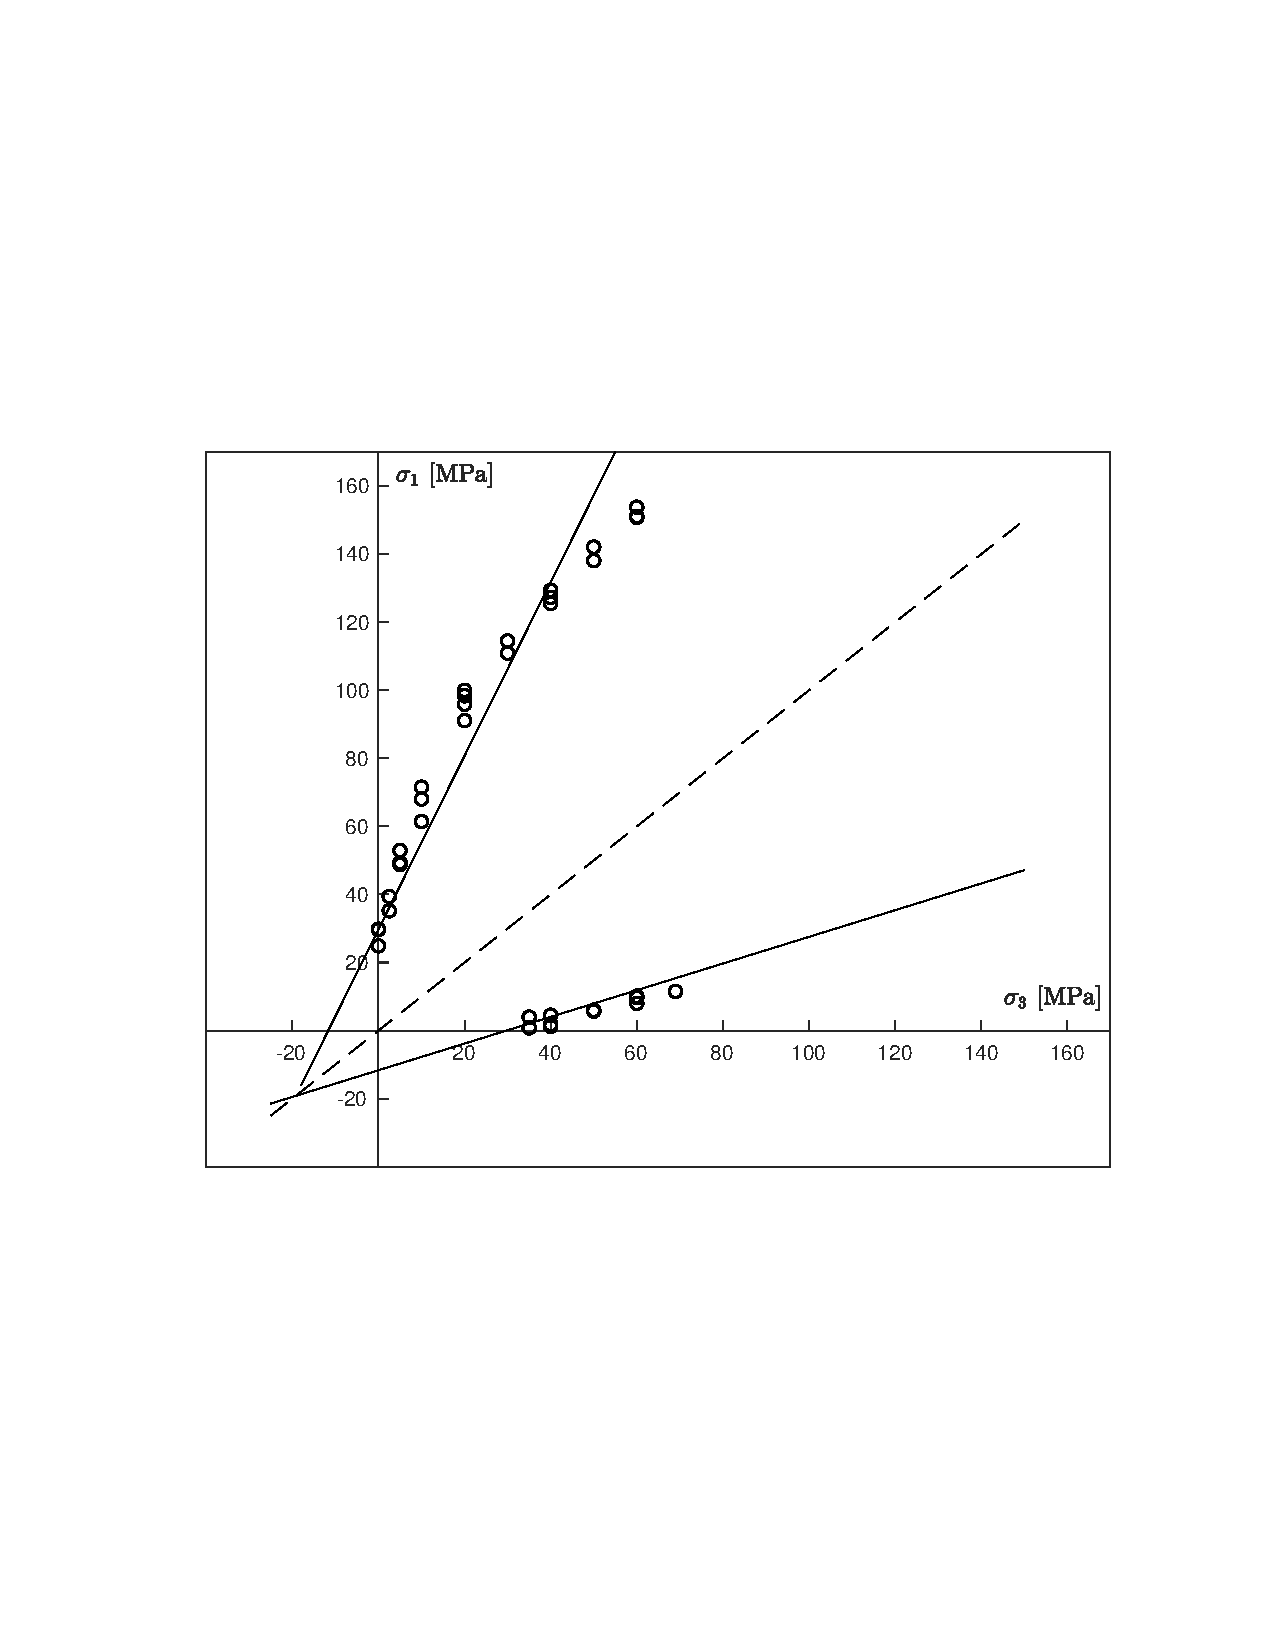
\includegraphics[width=0.7\columnwidth]{ch5/mc_sig1sig3}
    \caption{Mohr-Coulomb criterion failure surface in  $(\sigma_3-\sigma_1)$ plane}
    \label{fig5:mc_sig1sig3}
\end{figure} 

The criterion was also fitted in the $(p-q)$ plane, for which the plot obtained is shown in Figure \ref{fig5:mc_pq}. The coefficients $m_{c,e}$ and $b_{c,e}$ were computed using Equations \ref{eq2:MC_mc_q} to \ref{eq2:MC_be_q}:

\begin{equation}
    m_c = \frac{6 \sin \phi}{3-\sin \phi} = 1.02
\end{equation}
\begin{equation}
    m_e = \frac{6 \sin \phi}{3+\sin \phi} = 0.76
\end{equation}
\begin{equation}
    b_c = \frac{6 c \cos \phi}{3-\sin \phi} = \SI{19.6}{\mega\pascal}
\end{equation}
\begin{equation}
    b_e = \frac{6 c \cos \phi}{3+\sin \phi} = \SI{14.6}{\mega\pascal}
\end{equation}

\begin{figure}[p]
    \centering
    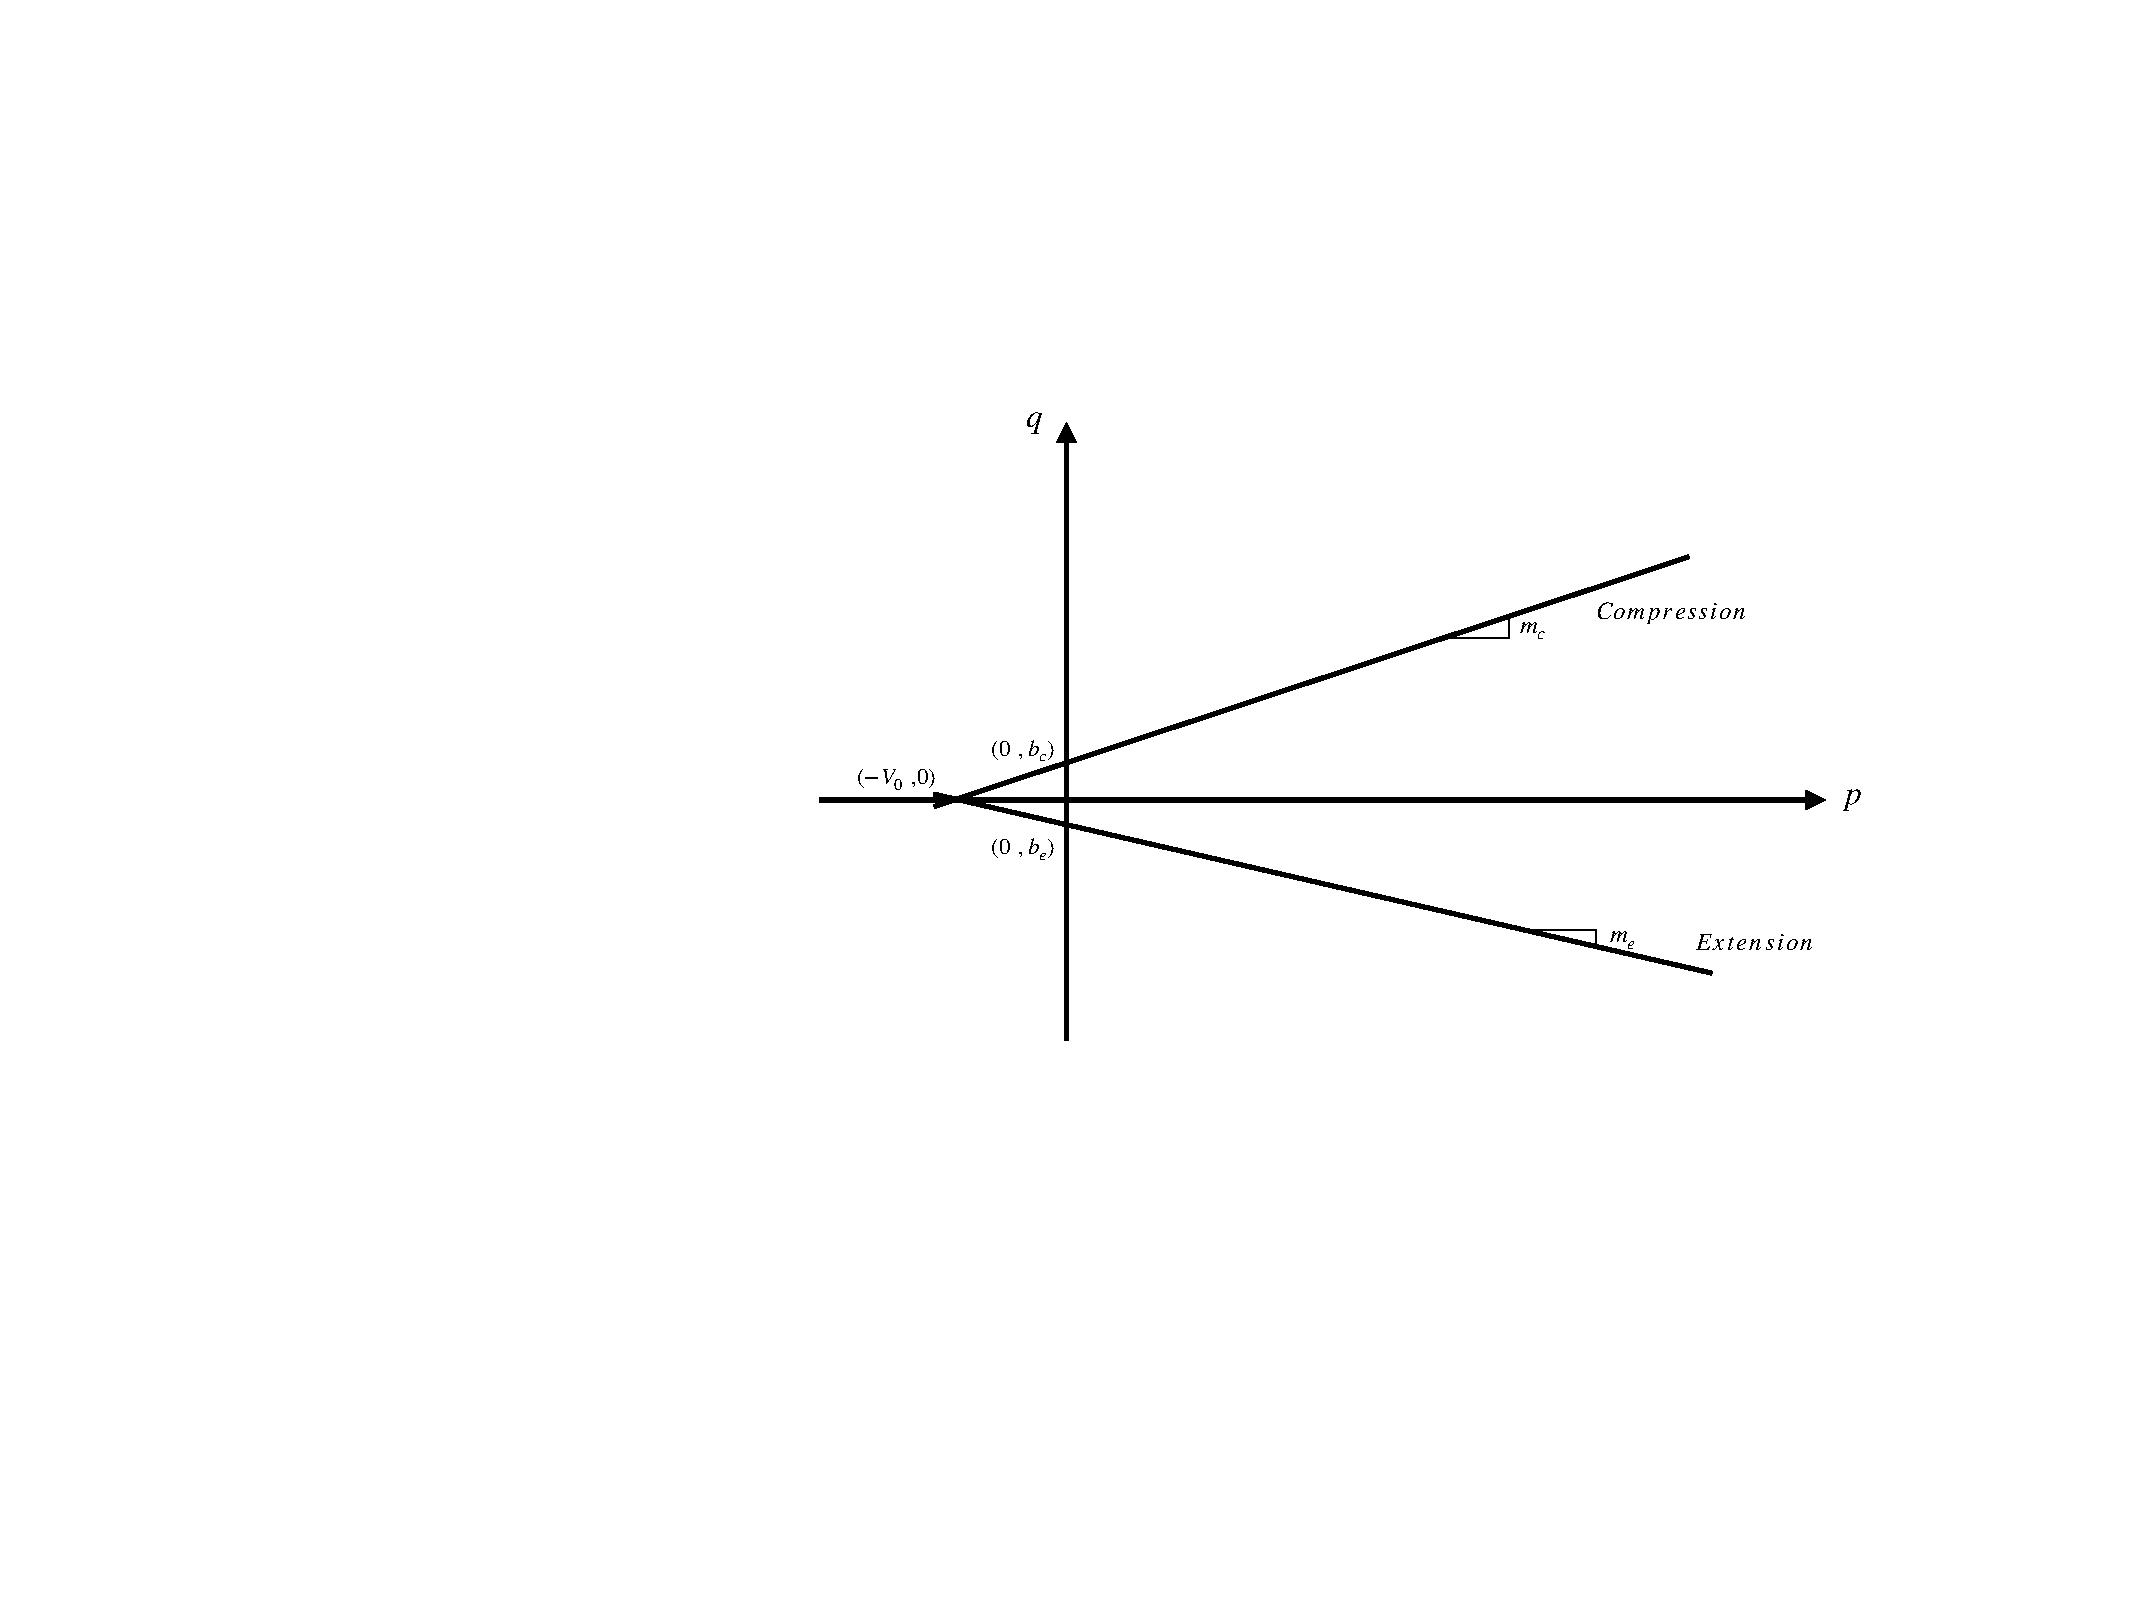
\includegraphics[width=0.7\columnwidth]{ch5/mc_pq}
    \caption{Mohr-Coulomb criterion failure surface in  $(p-q)$ plane}
    \label{fig5:mc_pq}
\end{figure} 

Finally, the Mohr-Coulomb criterion is presented in the $\pi$-plane, obtained following the procedure described in Section \ref{ch2:MC_pi}. Figure \ref{fig5:mc_pi_plane} shows Mohr-Coulomb failure criterion in the pi-plane at different values of the mean stress $p$.

\begin{figure}[tb]
    \centering
    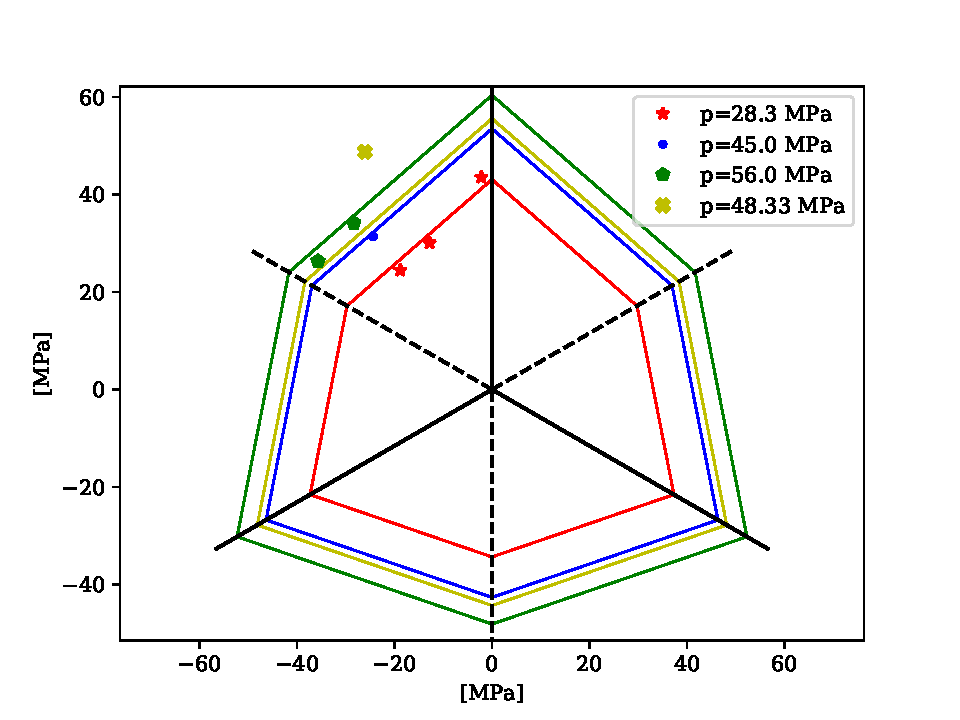
\includegraphics[width=0.5\columnwidth]{ch5/mc_pi_plane1}
    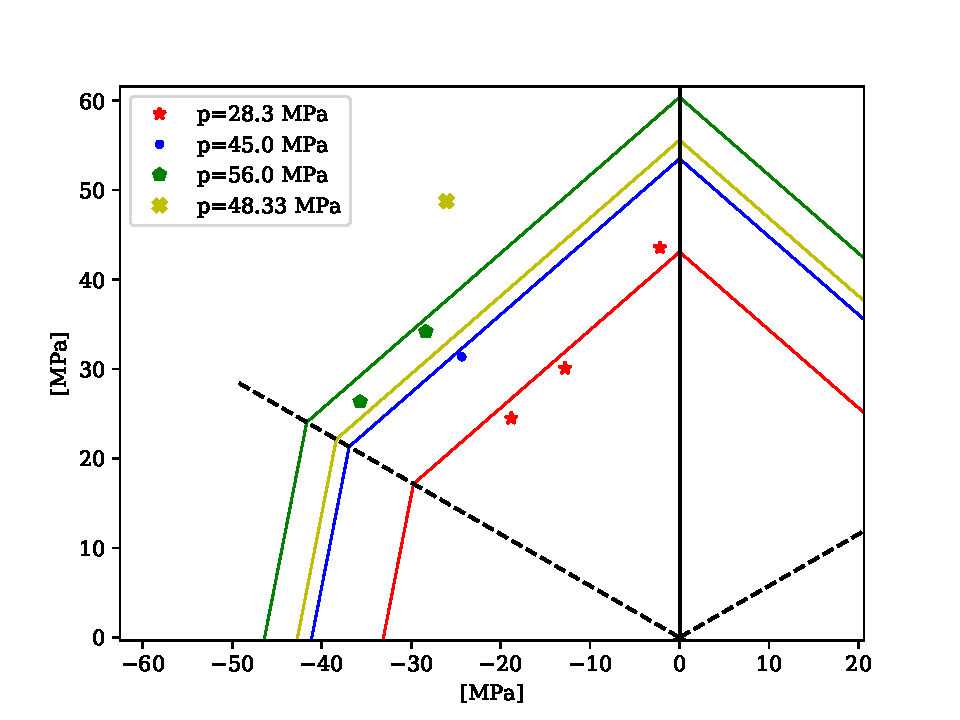
\includegraphics[width=0.8\columnwidth]{ch5/mc_pi_plane2}
    \caption{Mohr-Coulomb criterion failure surface in  $\pi$-plane}
    \label{fig5:mc_pi_plane}
\end{figure} 

The mean standard deviation misfit obtained with the Mohr-Coulomb failure criterion is $14.0$ \si{\mega\pascal}. 

%%%%%%%%%%%%%%%%%%%%%%%%%%%%%%%%%%%%%%%%%%%%%%%%%%%%%%%%%%%%%%
\subsection{Hoek-Brown failure criterion}

The Hoek-Brown failure criterion is also formulated in terms two principal stresses (cf. Equations \ref{eq2:HB-crit}) and unique strength parameters (i.e. $m$, $C_0$). Therefore, the fitting was done using only axisymmetric triaxial compression tests results (i.e. $\theta = 0^\circ$). 

From this fitting, the strength parameter $m$ was determined and $V_0$ was computed: 

\begin{equation}
    m = 5.96 \quad \textrm{and} \quad C_0 = \SI{29.7}{\mega\pascal}
\end{equation}
\begin{equation}
    V_0 = \frac{C_0}{m} = \SI{4.98}{\mega\pascal}
\end{equation}

Knowing the strength parameters, the Hoek-Brown failure surface is plotted in the $(\sigma_3-\sigma_1)$ plane using Equations \ref{eq2:HBsig1_CTC} for the compression line and \ref{eq2:HBsig1_CTE} for extension (cf. Figure \ref{fig5:mc_sig1sig3}).

\begin{figure}[p]
    \centering
    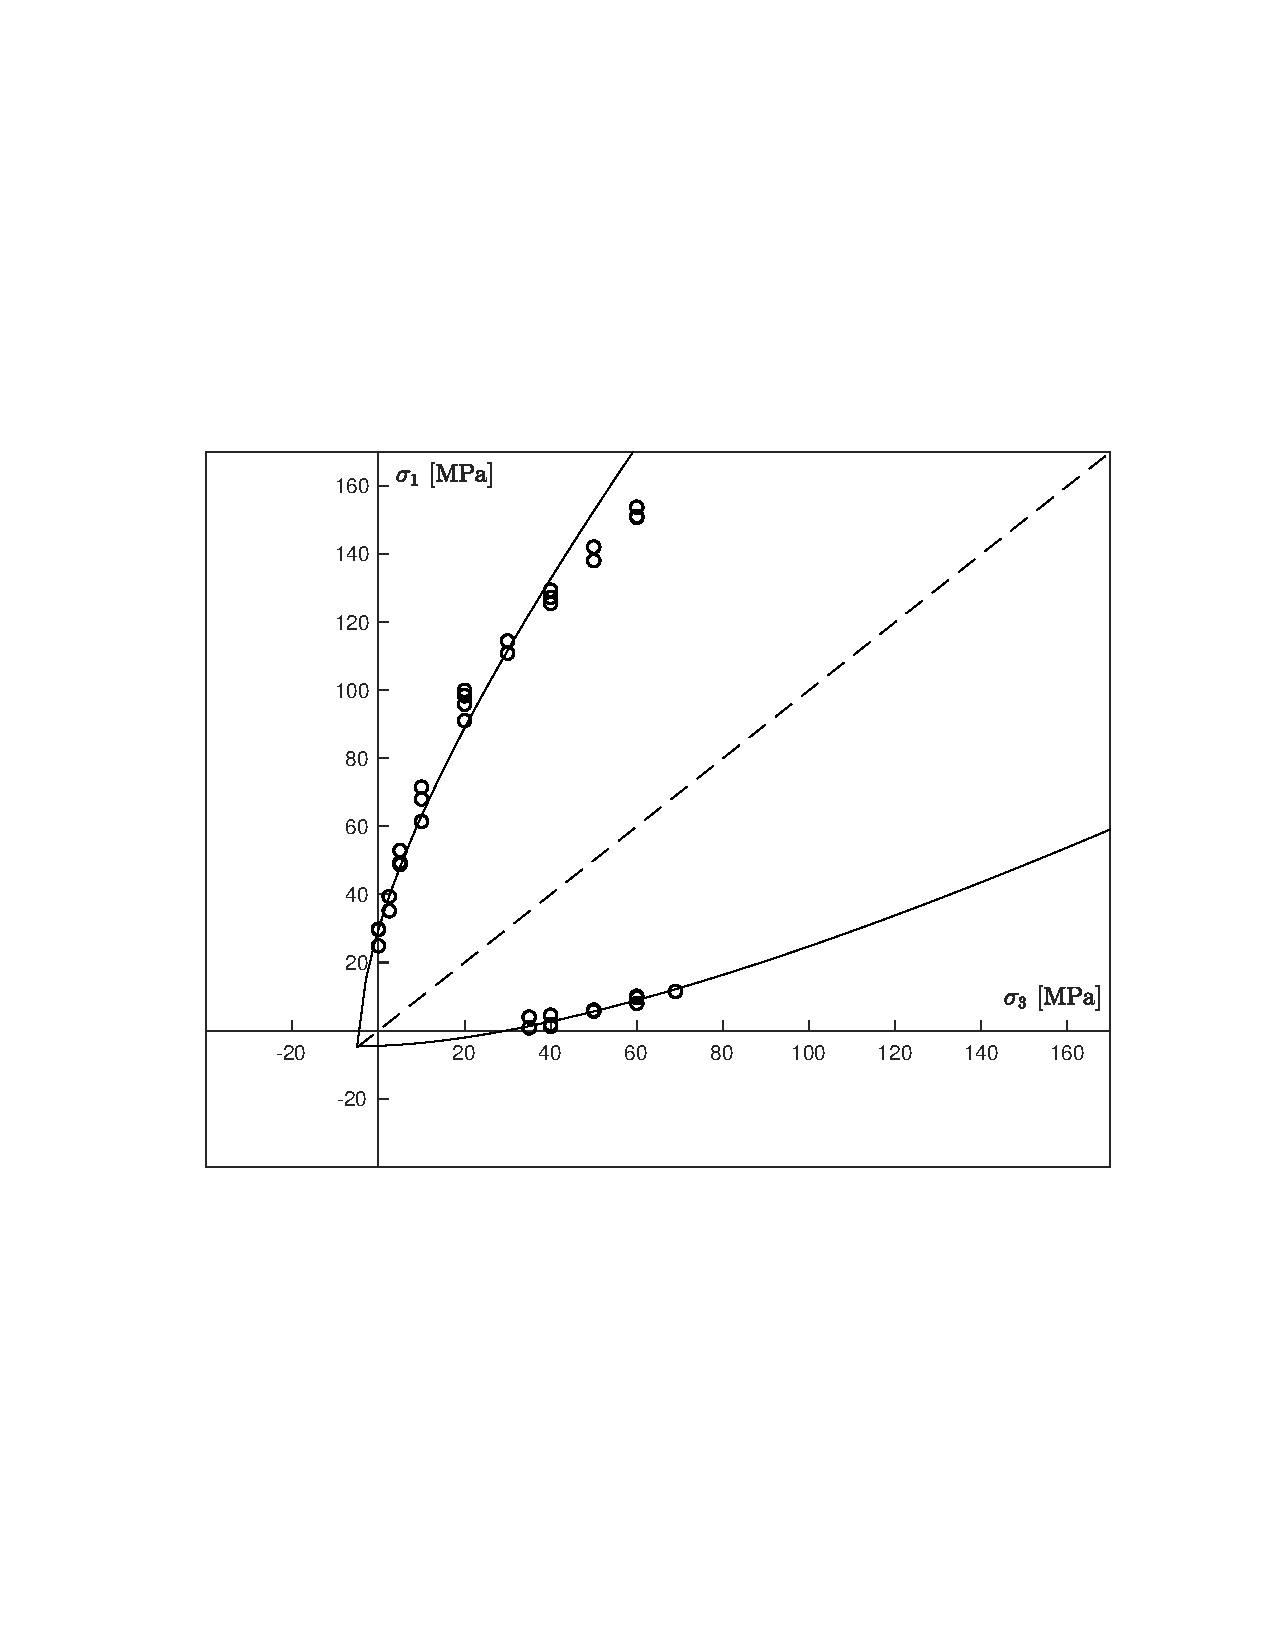
\includegraphics[width=0.7\columnwidth]{ch5/hb_sig1sig3}
    \caption{Hoek-Brown criterion failure surface in  $(\sigma_3-\sigma_1)$ plane}
    \label{fig5:hb_sig1sig3}
\end{figure} 

In the $(p-q)$ plane, the Hoek-Brown failure criterion is plotted using Equations \ref{eq2:HB-q-CTC} for compression and \ref{eq2:HB-q-CTE} for extension, and showed in Figure \ref{fig5:hb_pq}. These surfaces are expressed in terms of $m$ and $C_0$ previously defined. 

\begin{figure}[p]
    \centering
    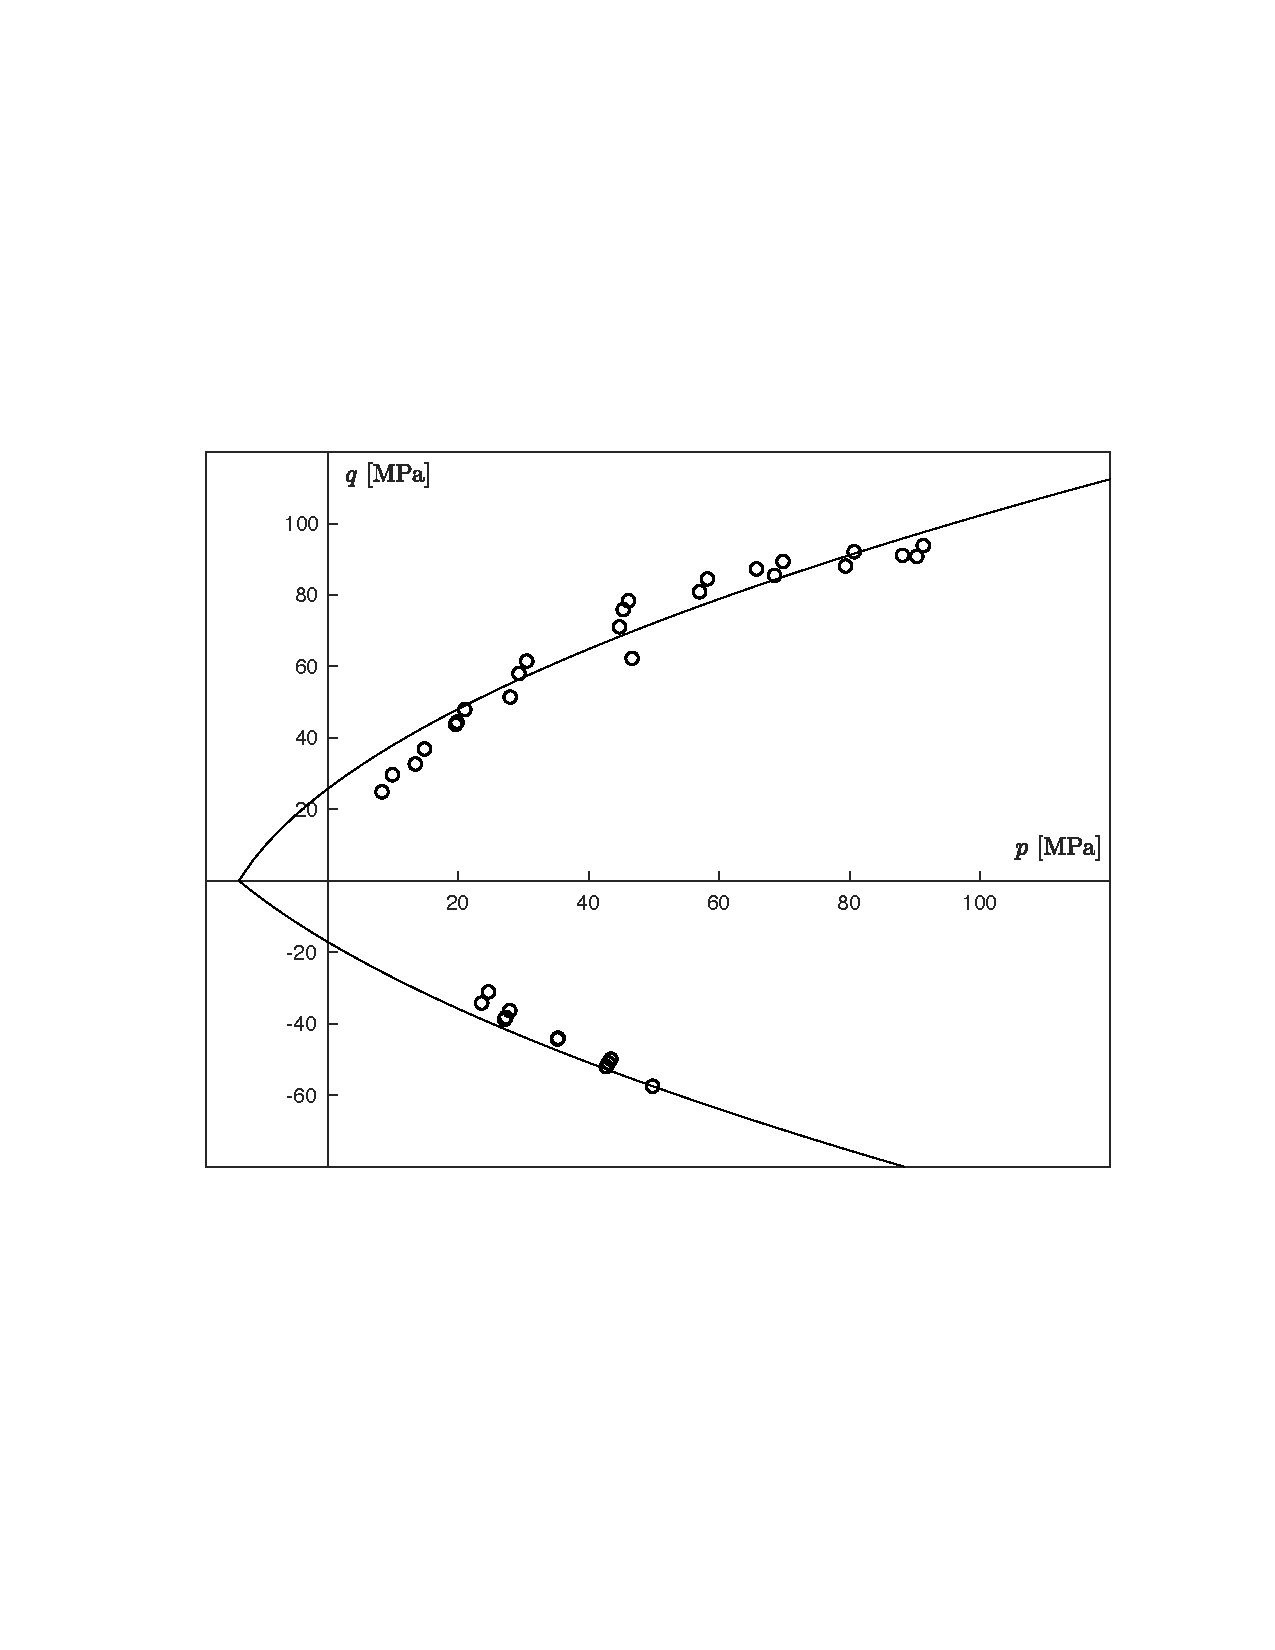
\includegraphics[width=0.7\columnwidth]{ch5/hb_pq}
    \caption{Hoek-Brown criterion failure surface in  $(p-q)$ plane}
    \label{fig5:hb_pq}
\end{figure} 

Finally, the Hoek-Brown criterion is presented in the $\pi$-plane, obtained following the procedure described in Section \ref{ch2:HB_pi}. Figure \ref{fig5:hb_pi_plane} shows Hoek-Brown failure criterion in the pi-plane at different values of the mean stress $p$.

\begin{figure}[tb]
    \centering
    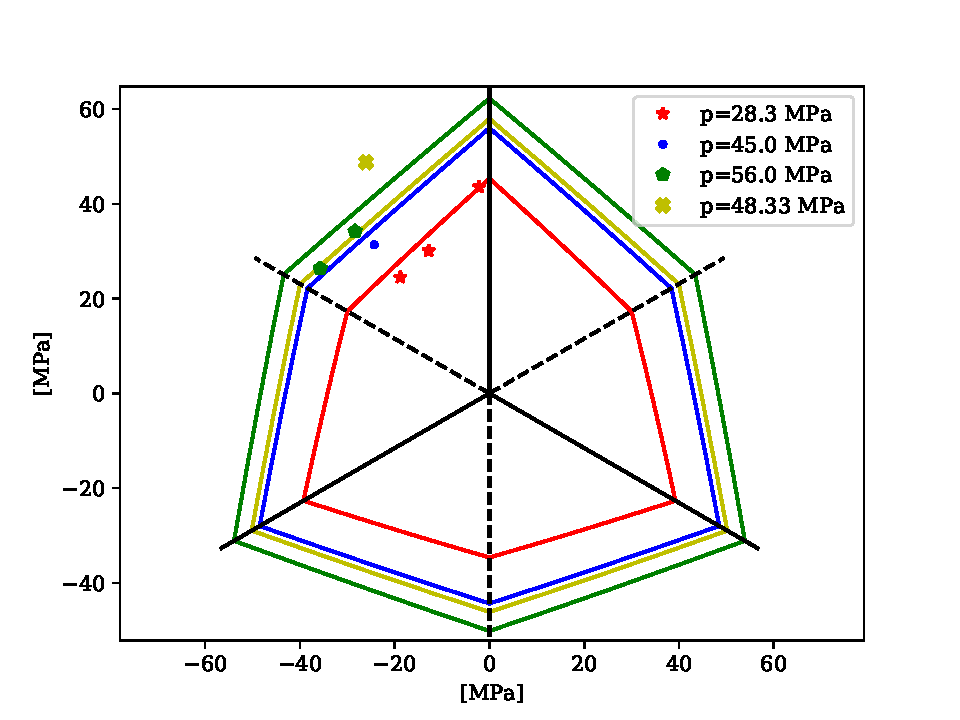
\includegraphics[width=0.5\columnwidth]{ch5/hb_pi_plane1}
    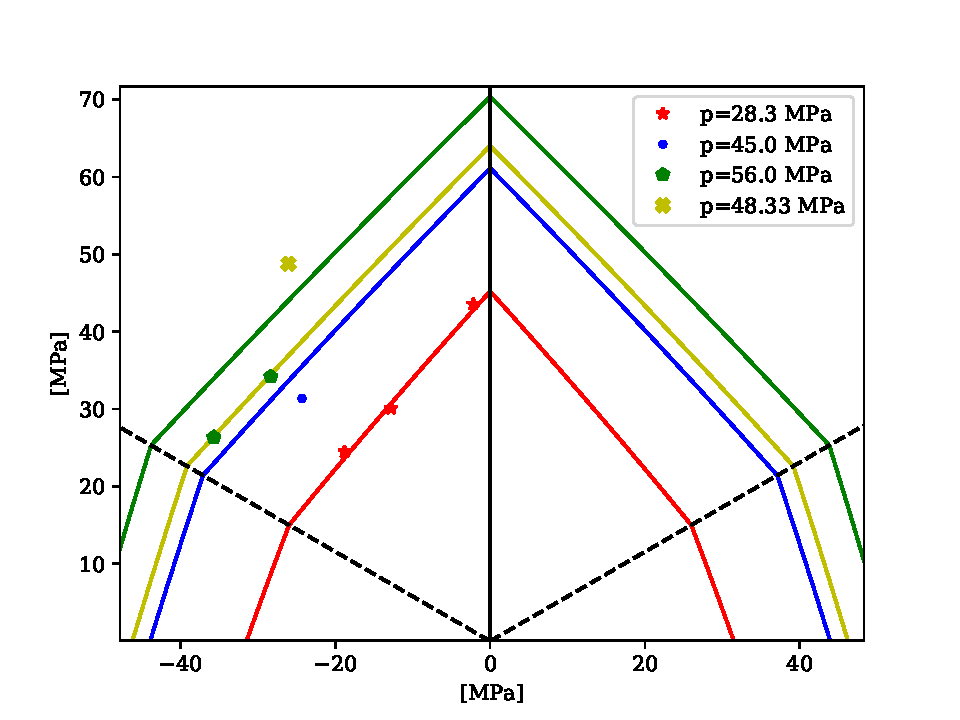
\includegraphics[width=0.8\columnwidth]{ch5/hb_pi_plane2}
    \caption{Hoek-Brown criterion failure surface in  $\pi$-plane}
    \label{fig5:hb_pi_plane}
\end{figure} 

The mean standard deviation misfit obtained with the Hoek-Brown failure criterion is $9.37$ \si{\mega\pascal}. 

%%%%%%%%%%%%%%%%%%%%%%%%%%%%%%%%%%%%%%%%%%%%%%%%%%%%%%%%%%%%%%
\subsection{Paul-Mohr-Coulomb failure criterion}\label{ch5:3p_pmc}

Contrary to the previous criteria, the Paul-Mohr-Coulomb failure criterion is formulated in terms the three principal stresses (cf. Equations \ref{eq2:PMC} and \ref{eq2:PMC_dev}) and non-unique strength parameters (i.e. $\phi_{c,e}$, $c_{c,e}$, $V_0$). Therefore, the fitting was done using all tests results from the database. 

From the least-square solution fitting describe in Chapter 2 (cf. Section \ref{ch2:pmcfit}, Equations \ref{eq2:PMCfinalform} and \ref{eq2:pmc_be}), the following solution could be obtained:
\begin{equation}
    x_1 = \frac{b_c}{V_0} = 0.81
\end{equation}
\begin{equation}
    x_2 = k = -0.91
\end{equation}
\begin{equation}\label{eq5:pmc_bc}
    x_3 = b_c = \SI{28.77}{\mega\pascal}
\end{equation}

Following Equations \ref{eq2:pmc_vo} to \ref{eq2:pmc_c}, the strength parameters for Paul-Mohr-Coulomb failure criteria could be computed:

\begin{equation}
    V_0 = \frac{0.81}{b_c} = \SI{35.62}{\mega\pascal}
\end{equation}
\begin{equation}\label{eq5:pmc_be}
    b_e = \frac{2b_c}{(1-\sqrt{3}k)} = \SI{22.31}{\mega\pascal}
\end{equation}
\begin{equation}
    \phi_c = arcsin\left(\frac{3b_c}{6V_0+b_c}\right) = \SI{20.85}{\degree}
\end{equation}
\begin{equation}
    \phi_e = arcsin\left(\frac{3b_e}{6V_0-b_c}\right) = \SI{20.85}{\degree}
\end{equation}
\begin{equation}
    c_{c}=\frac{b_{c}\left(3-\sin \phi_{c}\right)}{6 \cos \phi_{c}} = \SI{13.57}{\mega\pascal}
\end{equation}
\begin{equation}
    c_{e}=\frac{b_{e}\left(3+\sin \phi_{e}\right)}{6 \cos \phi_{e}} = \SI{10.52}{\mega\pascal}
\end{equation}

Knowing the strength parameters, the Paul-Mohr-Coulomb failure surface could be plotted in the $(\sigma_3-\sigma_1)$ plane using Equations \ref{eq2:PMC_sig1sig3} to \ref{eq2:PMC_sig1sig3_Cce}. The graph obtained, using the coefficients computed in Equations \ref{eq5:pmc_Mc} to \ref{eq5:pmc_Ce}, is presented in Figure \ref{fig5:pmc_sig1sig3}.

\begin{equation}\label{eq5:pmc_Mc}
    M_c = \frac{1+\sin \phi_c}{1-\sin \phi_c} = 2.11
\end{equation}
\begin{equation}
    M_e = \frac{1+\sin \phi_e}{1-\sin \phi_e} = 2.08
\end{equation}
\begin{equation}
    C_c = \frac{2c_c\cos \phi_c}{1-\sin \phi_c} = \SI{39.38}{\mega\pascal}
\end{equation}
\begin{equation}\label{eq5:pmc_Ce}
    C_e = \frac{2c_e\cos \phi_e}{1-\sin \phi_e} = \SI{30.31}{\mega\pascal}
\end{equation}

\begin{figure}[p]
    \centering
    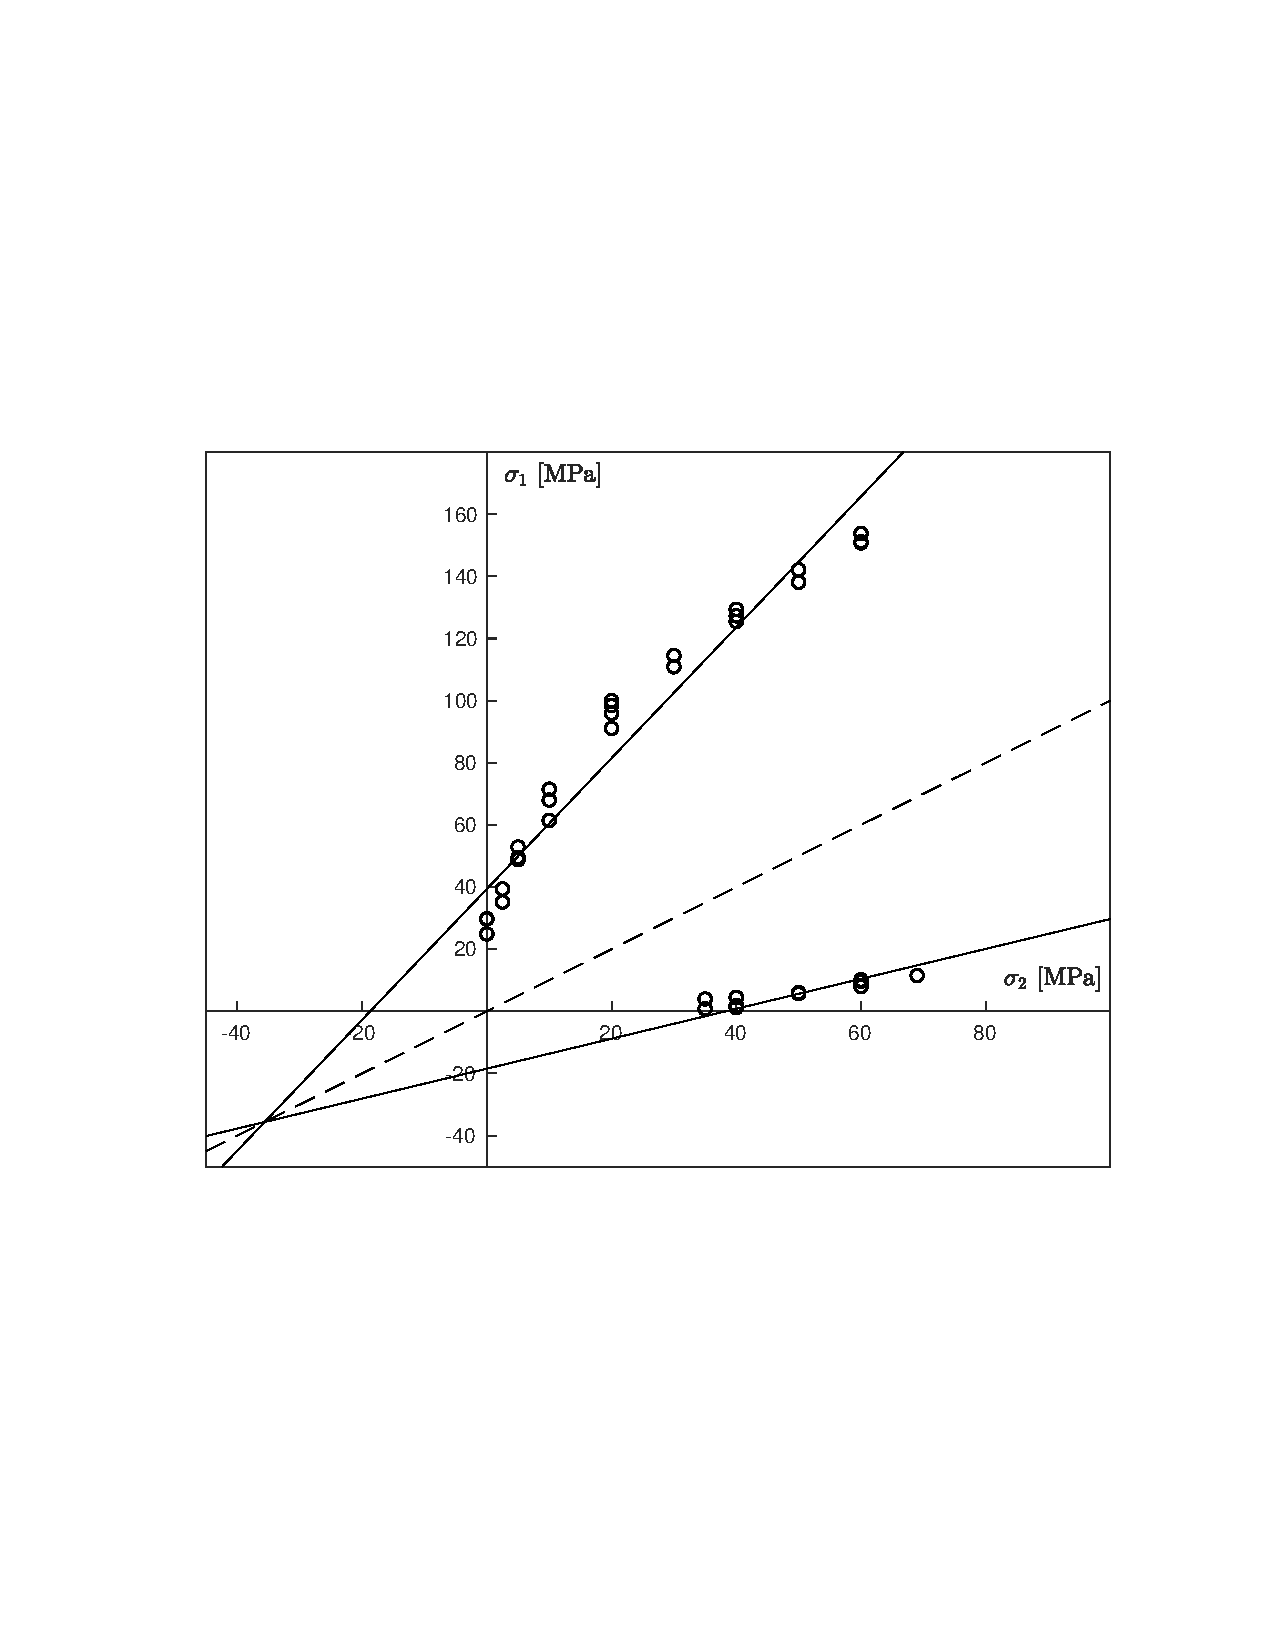
\includegraphics[width=0.7\columnwidth]{ch5/pmc3p_sig1sig3}
    \caption{Paul-Mohr-Coulomb criterion failure surface in  $(\sigma_3-\sigma_1)$ plane}
    \label{fig5:pmc_sig1sig3}
\end{figure}

In the $(p-q)$ plane, the Paul-Mohr-Coulomb failure criterion is plotted using Equations \ref{eq2:PMC_pq} to \ref{eq2:pmc_b_pq}, and the graph obtained in presented in Figure \ref{fig5:pmc_pq}. These surfaces are expressed in terms of $b_{c,e}$,defined by Equations \ref{eq5:pmc_bc} and \ref{eq5:pmc_be}, and $m_{c,e}$ computes as follow: 

\begin{equation}\label{eq5:pmc_mc}
    m_c=\frac{6 \sin \phi_{c}}{3-\sin \phi_{c}} = 0.81
\end{equation}
\begin{equation}\label{eq5:pmc_me}
    m_e=\frac{6 \sin \phi_{e}}{3-\sin \phi_{e}} = 0.63
\end{equation}

\begin{figure}[p]
    \centering
    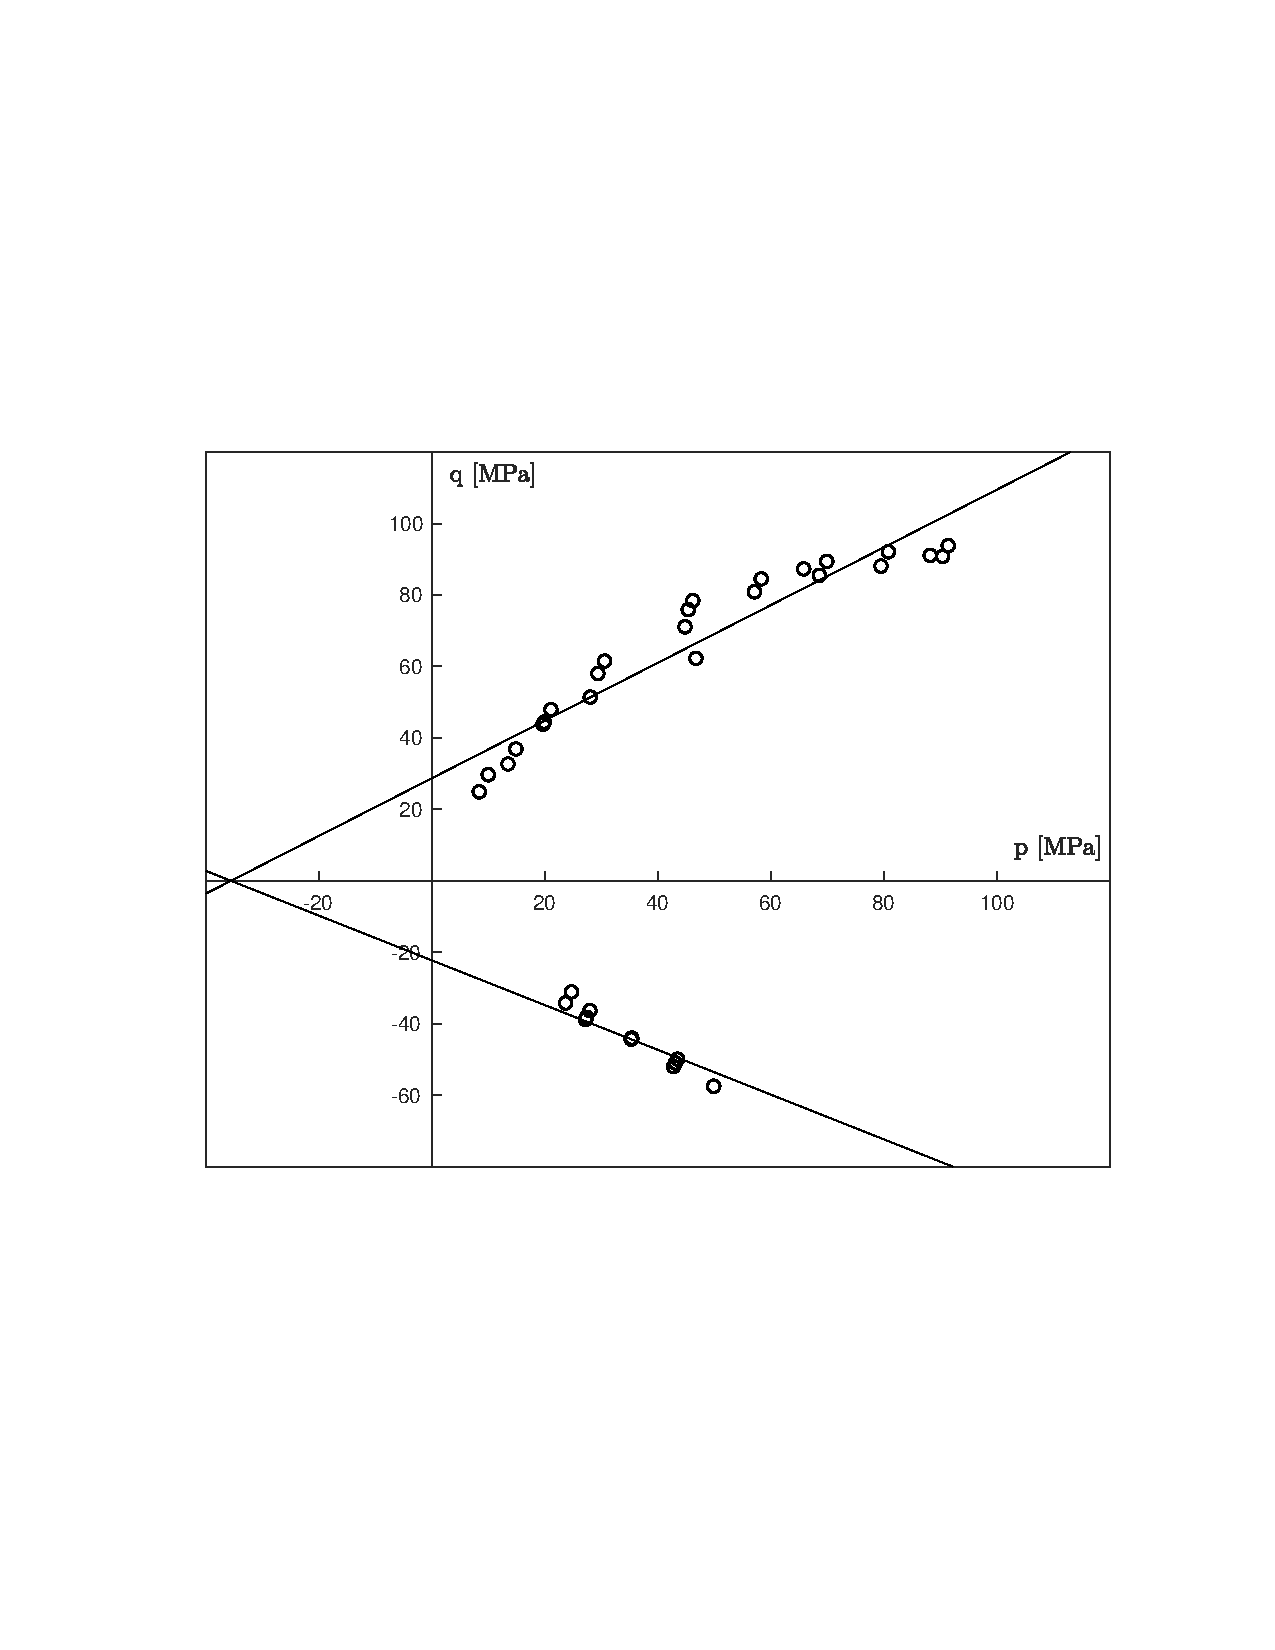
\includegraphics[width=0.7\columnwidth]{ch5/pmc3p_pq}
    \caption{Paul-Mohr-Coulomb criterion failure surface in $(p-q)$ plane}
    \label{fig5:pmc_pq}
\end{figure} 

Finally, the Paul-Mohr-Coulomb criterion is presented in the $\pi$-plane, obtained following the procedure described in Section \ref{ch2:PMC}. Figure \ref{fig5:pmc_pi_plane} shows the failure criterion in the $\pi$-plane at different mean stresses $p$, corresponding to true-triaxial experiments mean stresses at failure (i.e. data points where $0^\circ < \theta < 60^\circ$ in Table \ref{tb5:database}).

\begin{figure}[tb]
    \centering
    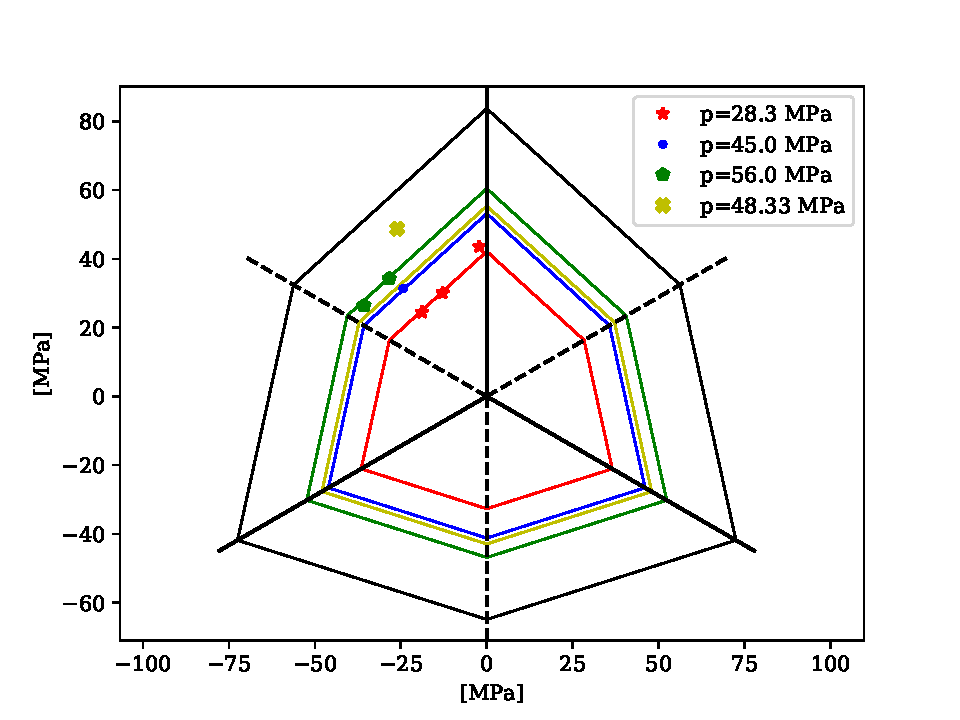
\includegraphics[width=0.5\columnwidth]{ch5/pmc3p_pi_pts1}
    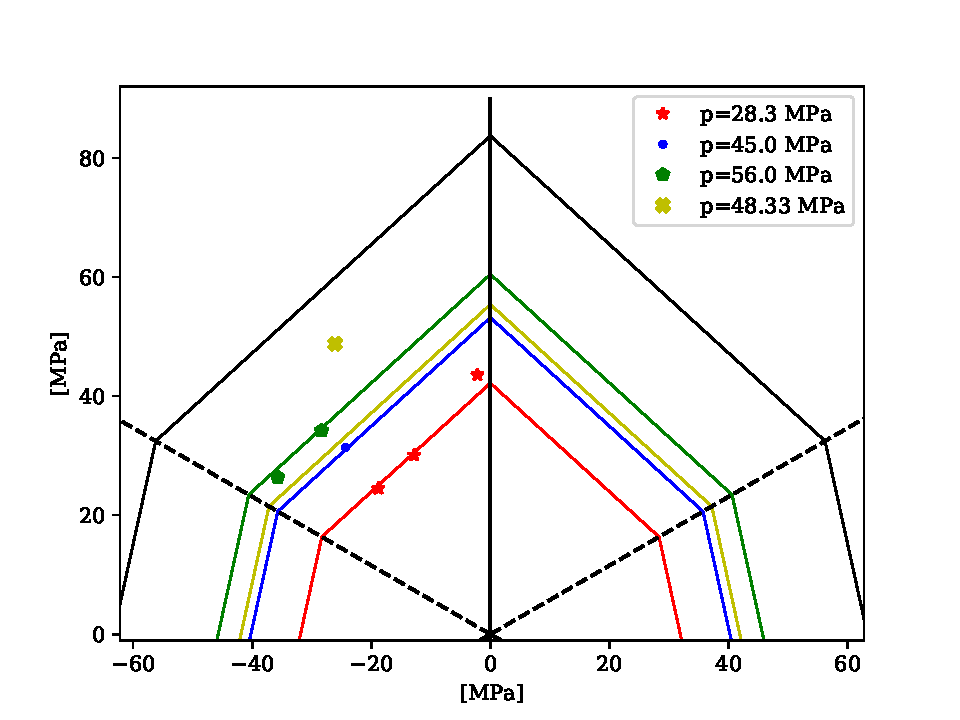
\includegraphics[width=0.8\columnwidth]{ch5/pmc3p_pi_pts2}
    \caption{Paul-Mohr-Coulomb criterion failure surface in  $\pi$-plane}
    \label{fig5:pmc_pi_plane}
\end{figure} 

The mean standard deviation misfit obtained with the Paul-Mohr-Coulomb failure criterion is $13.2$ \si{\mega\pascal}. 

%%%%%%%%%%%%%%%%%%%%%%%%%%%%%%%%%%%%%%%%%%%%%%%%%%%%%%%%%%%%%%
\subsection{Comparison of the failure criteria}

The mean standard deviation misfits obtained for the three failure criteria show that Hoek-Brown provides a better approximation of the data points (cf. Table \ref{tb5:stand_dev}). However, it should be kept in mind that this criterion was fitted only for data points related to axisymmetric compression experiments. Therefore, its prediction of true triaxial experiments is less accurate than the one provided by the Paul-Mohr-Coulomb criterion. This can be easily noticed with the observation of both predictions in the $\pi$-plane (cf. Figures \ref{fig5:hb_pi_plane} and \ref{fig5:pmc_pi_plane}). 

\begin{table}
    \centering
    \begin{tabular}{ccc}
        \hline 
        Criterion & Mean standard deviation misfit $\bar{S}$ []\si{MPa}] \\
        \hline
        \hline
        Mohr-Coulomb & 14.0 \\
        Hoek-Brown & 9.37 \\
        Paul-Mohr-Coulomb & 13.2 \\
        \hline
    \end{tabular}
    \captionsetup{justification=centering}
    \caption{Summary of the mean standard deviation misfits obtained for the three failure criteria evaluated}
    \label{tb5:stand_dev}
\end{table}

%%%%%%%%%%%%%%%%%%%%%%%%%%%%%%%%%%%%%%%%%%%%%%%%%%%%%%%%%%%%%%%%%%%%%%%%%%%%%%%%%%%%%%%%%%%%%%%%%%%%%%%%%%%%%%%%%%%%%%%%%%%%%%%%%%%%%%%%%%%
\section{Bi-linear Paul-Mohr-Coulomb failure criterion}\label{ch5:PMC}

Published data from multi axial experiments on multiple rocks showed that the failure envelop that describe them best is not linear over a large range of mean stress. However, popular failure theories as Mohr-Coulomb or Hoek-Brown, are either linear or do not provide an accurate prediction for all mean stresses. In this study, Paul-Mohr-Coulomb failure criteria is chosen to address this issue by approximating the nonlinear failure surface in a piecewise linear manner, resulting in a failure surface defined by six parameters.

\subsection{Paul-Mohr-Coulomb with six parameters}\label{ch5:PMC_theo_6p}

The theoretical background on the six parameters Paul-Mohr-Coulom criterion presented in this section is based on the work of Labuz et al. (2018) \cite{Labuz2018}.

The Paul-Mohr-Coulomb failure criterion presented in the Section \ref{ch5:3p_pmc} is referred to as Paul-Mohr-Coulomb with three parameters, which failure surface is a plane defined by the general equation of the criterion (cf. Equation \ref{eq2:PMC_dev}), using three strength parameters : $V_0$, $\phi_c$ and $\phi_e$. The Paul-Mohr-Coulomb failure surface defined in a piecewise manner is, therefore, made of a minimum of two plane, each expressed using three strength parameters, leading to the six parameters criterion.

The three parameters criterion definition in terms of the three principal stresses describes a regular 6-sided pyramid in the principal stresses three-dimensional space (cf. Section \ref{ch2:background}). By adding a plane to the failure surface, the six parameters criterion, therefore, describes two irregular 6-sided pyramids. Each plane is then defined by the parameters presented in Table \ref{tb5:pmc6p_planeparam}, where $P2$ indicates the plane that approximate data points at low mean stress and $P1$ the ones at higher mean stress. Table \ref{tb5:pmc6p_pyramids} present four types of Paul-Mohr-Coulomb failure surfaces which can be defined according to the values of the parameters. For all types, the following conditions apply: 
\begin{equation}
    V_0^{(1)} > V_0^{(2)} \quad \textrm{and} \quad \SI{0}{\degree} \leq \phi_{c,e}^{(i)} \leq \SI{60}{\degree}
\end{equation}

\begin{table}
    \centering 
    \begin{tabular}{ccc}
        \hline 
        Plane & $P1$ & $P2$  \\
        \hline
        \hline
        Friction angle in compression & $\phi_{c}^{(1)}$ & $\phi_{c}^{(2)}$ \\
        \\
        Friction angle in extension & $\phi_{e}^{(1)}$ & $\phi_{e}^{(2)}$ \\ 
        \\
        Theoretical uniaxial tensile strength & $V_0^{(1)}$ & $V_0^{(2)}$ \\
        \hline
    \end{tabular}
    \captionsetup{justification=centering}
    \caption{Parameters of the planes defining the failure surface of Paul-Mohr-Coulomb criterion}
    \label{tb5:pmc6p_planeparam}
\end{table}

\begin{table}
    \centering 
    \begin{tabular}{cc}
        \hline 
        Type of failure surface & Parameters conditions   \\
        \hline
        \hline
        (i) 6-sided & $V_0^{(1)} = V_0^{(2)}$ \\
        \\
        (ii) 6-12-6 sided & $\phi_{c}^{(1)} < \phi_{c}^{(2)}$, $\phi_{e}^{(1)}$ < $\phi_{e}^{(2)}$, $p_c \neq p_e$\\ 
        \\
        (iii) 6-12 sided & ($\phi_{c}^{(1)} < \phi_{c}^{(2)}$, $\phi_{e}^{(1)} \geq \phi_{e}^{(2)}$) or ($\phi_{c}^{(1)} \geq \phi_{c}^{(2)}$, $\phi_{e}^{(1)} < \phi_{e}^{(2)}$)\\
        \\
        (iv) 6-12-6 sided & $\phi_{c}^{(1)} < \phi_{c}^{(2)}$, $\phi_{e}^{(1)}$ < $\phi_{e}^{(2)}$, $p_c = p_e$\\ 
        \hline
    \end{tabular}
    \captionsetup{justification=centering}
    \caption{Types of failure surfaces for the six parameters Paul-Mohr-Coulomb criterion}
    \label{tb5:pmc6p_pyramids}
\end{table}

The complete graphical representation of the Paul-Mohr-Coulomb failure surface is composed of the $(p-q)$ plane, the $(\sigma_2-\sigma_1)$ plane, the $\pi$-plane and the principal stresses three-dimensional space. The transition between $P2$ and $P1$ is well represented in the $(p-q)$ plane, where they intersect on the compression side (i.e. $q > 0$) at the mean stress value $p_c$ and on the extension side (i.e. $q < 0$) at $p_e$. In the case of the failure surface type (ii), these transitions points have different values leading to a 12 sided transition zone on the pyramid for mean stress values $p \in \left[p_c;p_e\right]$. Sketches of the 6-12-6 sided failure surface in different planes and in the three-dimensional space are presented in Figure \ref{fig5:6pmc_typeii}, where the $(\sqrt{3}p-\sigma^*)$ plane is equivalent to the $(p-q)$ plane. More schematic representations and details on the four failure surfaces types are provided in APPENDIX C REF{APPENDIX C}.

\begin{figure}
    \centering
    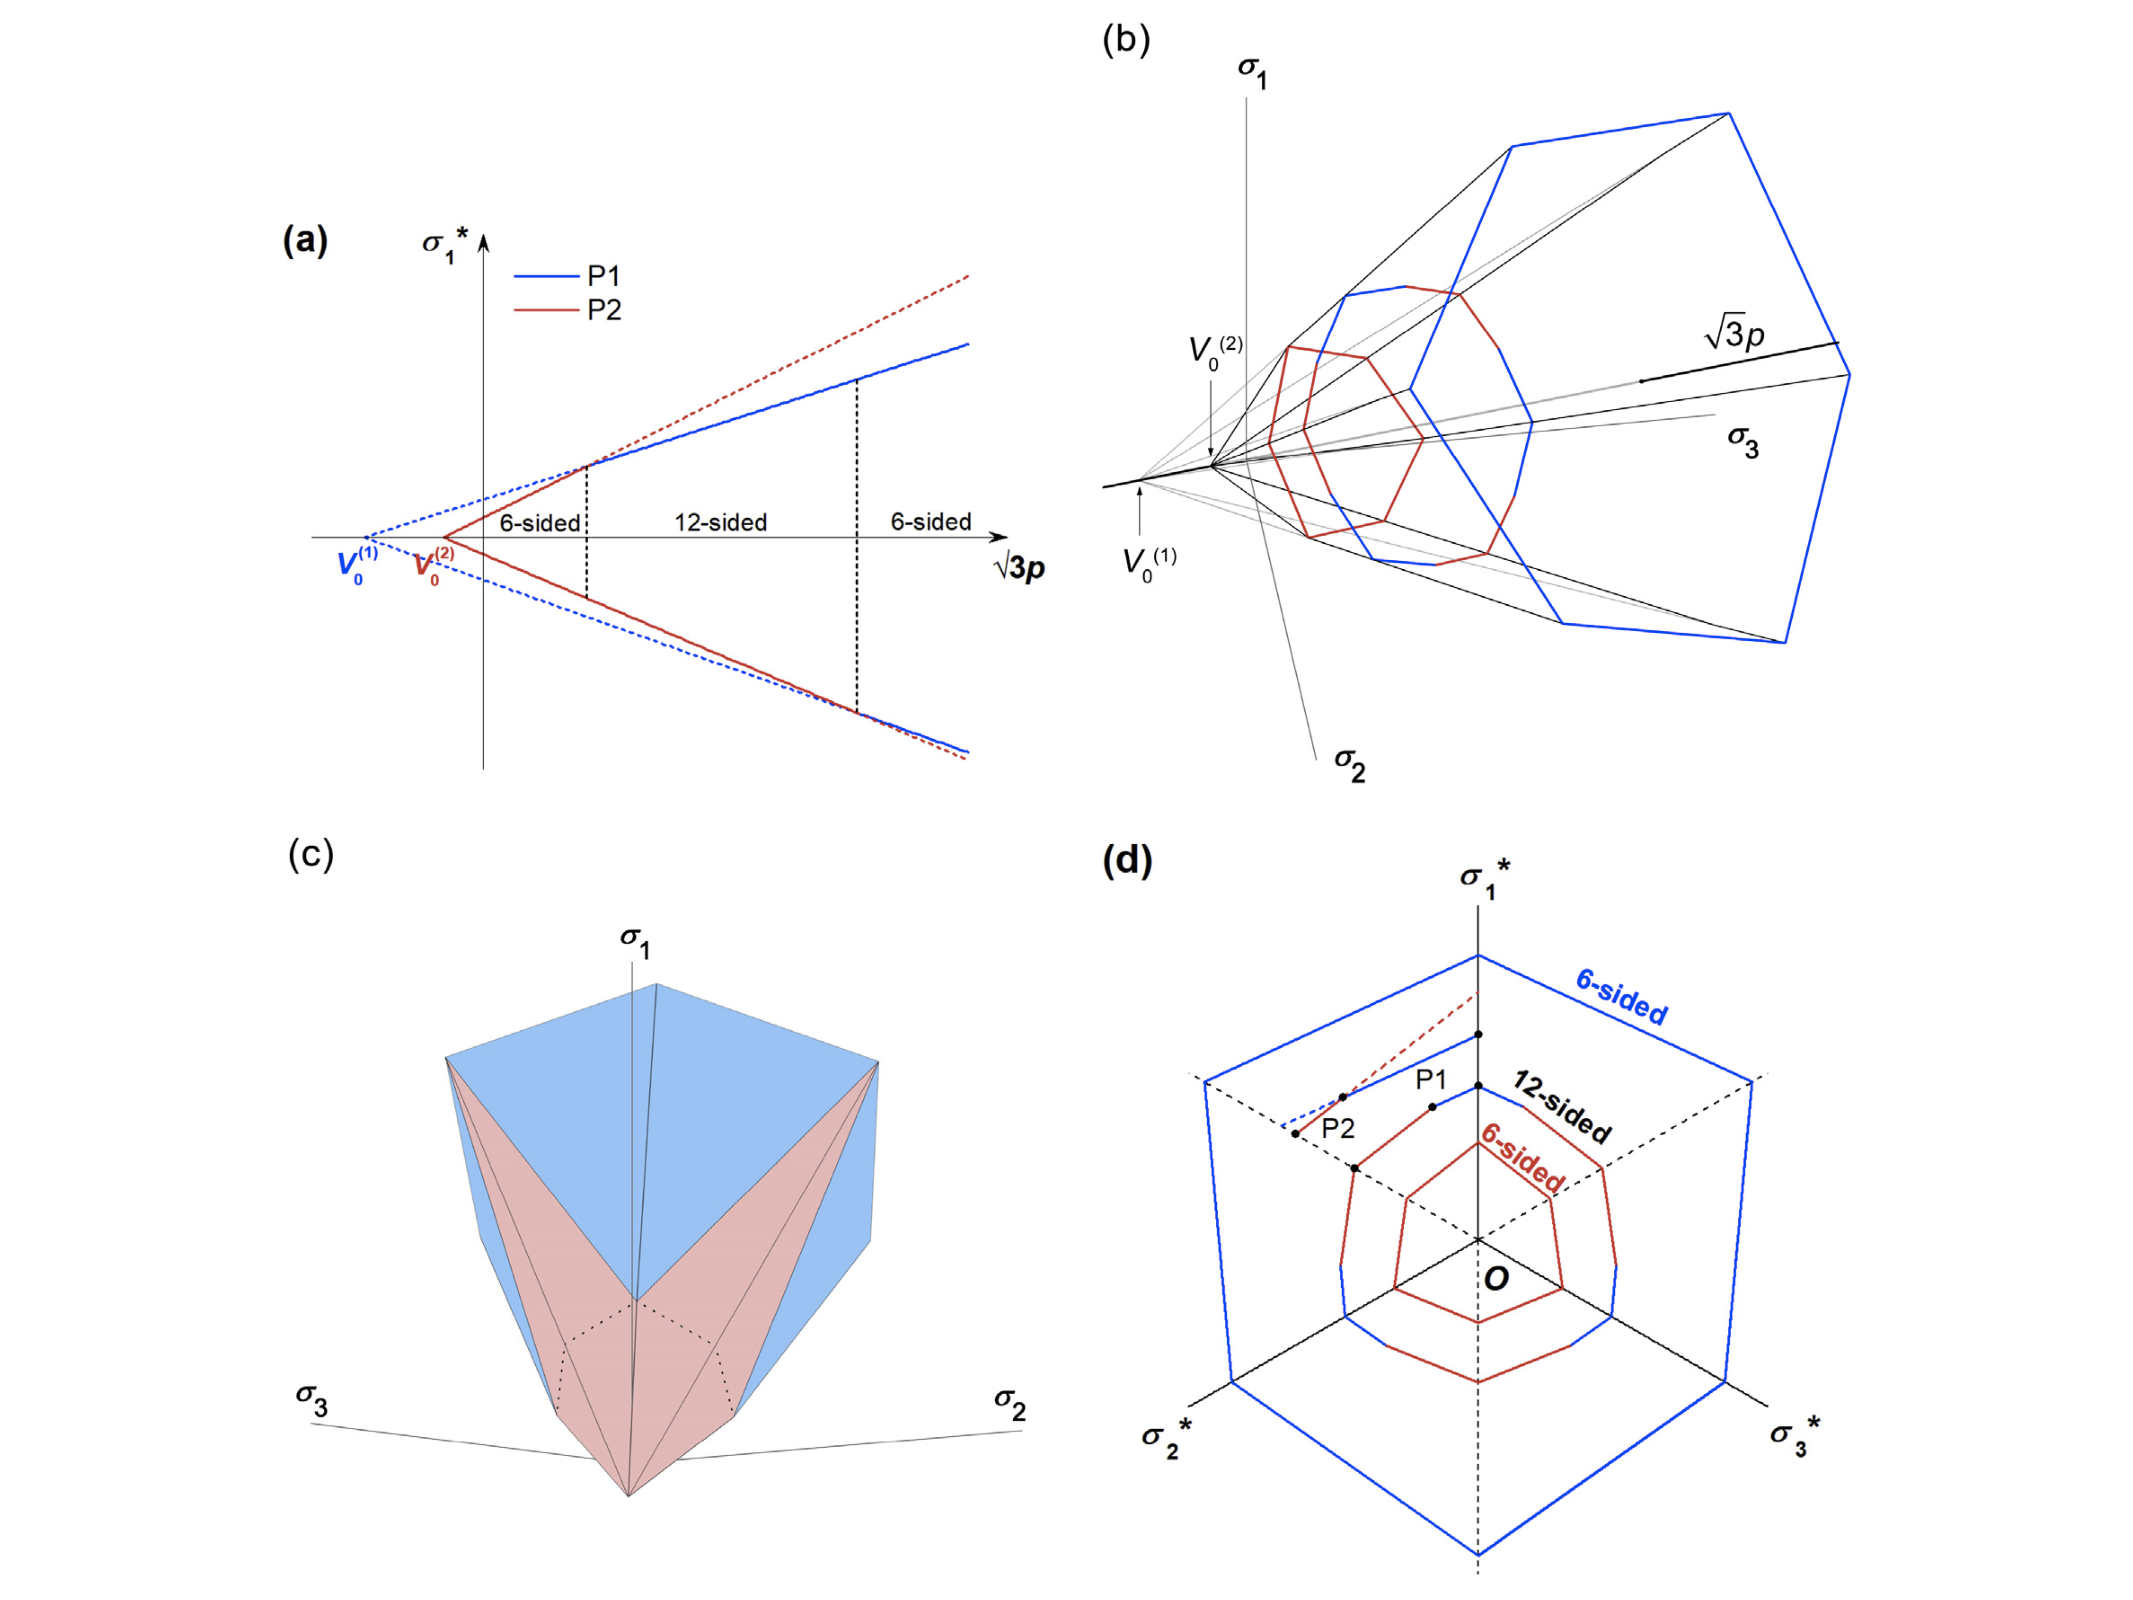
\includegraphics[width=\columnwidth]{ch5/pmc6_typeii}
    \caption{Paul-Mohr-Coulomb 6-12-6 sided failure surface graphical representations}
    \label{fig5:6pmc_typeii}
\end{figure}

The inclusion of the intermediate stress in the Paul-Mohr-Coulomb general equation (cf. Equation \ref{eq2:PMC}) makes relevant the representation of the criterion in the $(\sigma_2-\sigma_1)$ plane. Indeed, this plane presents the advantage to gather the data points for axisymmetric experiments, shown on compression and extension lines, as well as true-triaxial data in the same plot (cf. Figure \ref{fig5:6pmc_sig2sig1}). The Paul-Mohr-Coulomb failure surfaces are plotted for a chosen value of $\sigma_3$, using the following equation, based the rearrangement of Equation \ref{eq2:PMC}:

\begin{equation}\label{eq5:pmc_sig2sig1}
    \sigma_1 = \frac{1}{A}\left(1-B\sigma_{2}-C\sigma_{3}\right)
\end{equation}
\begin{figure}
    \centering
    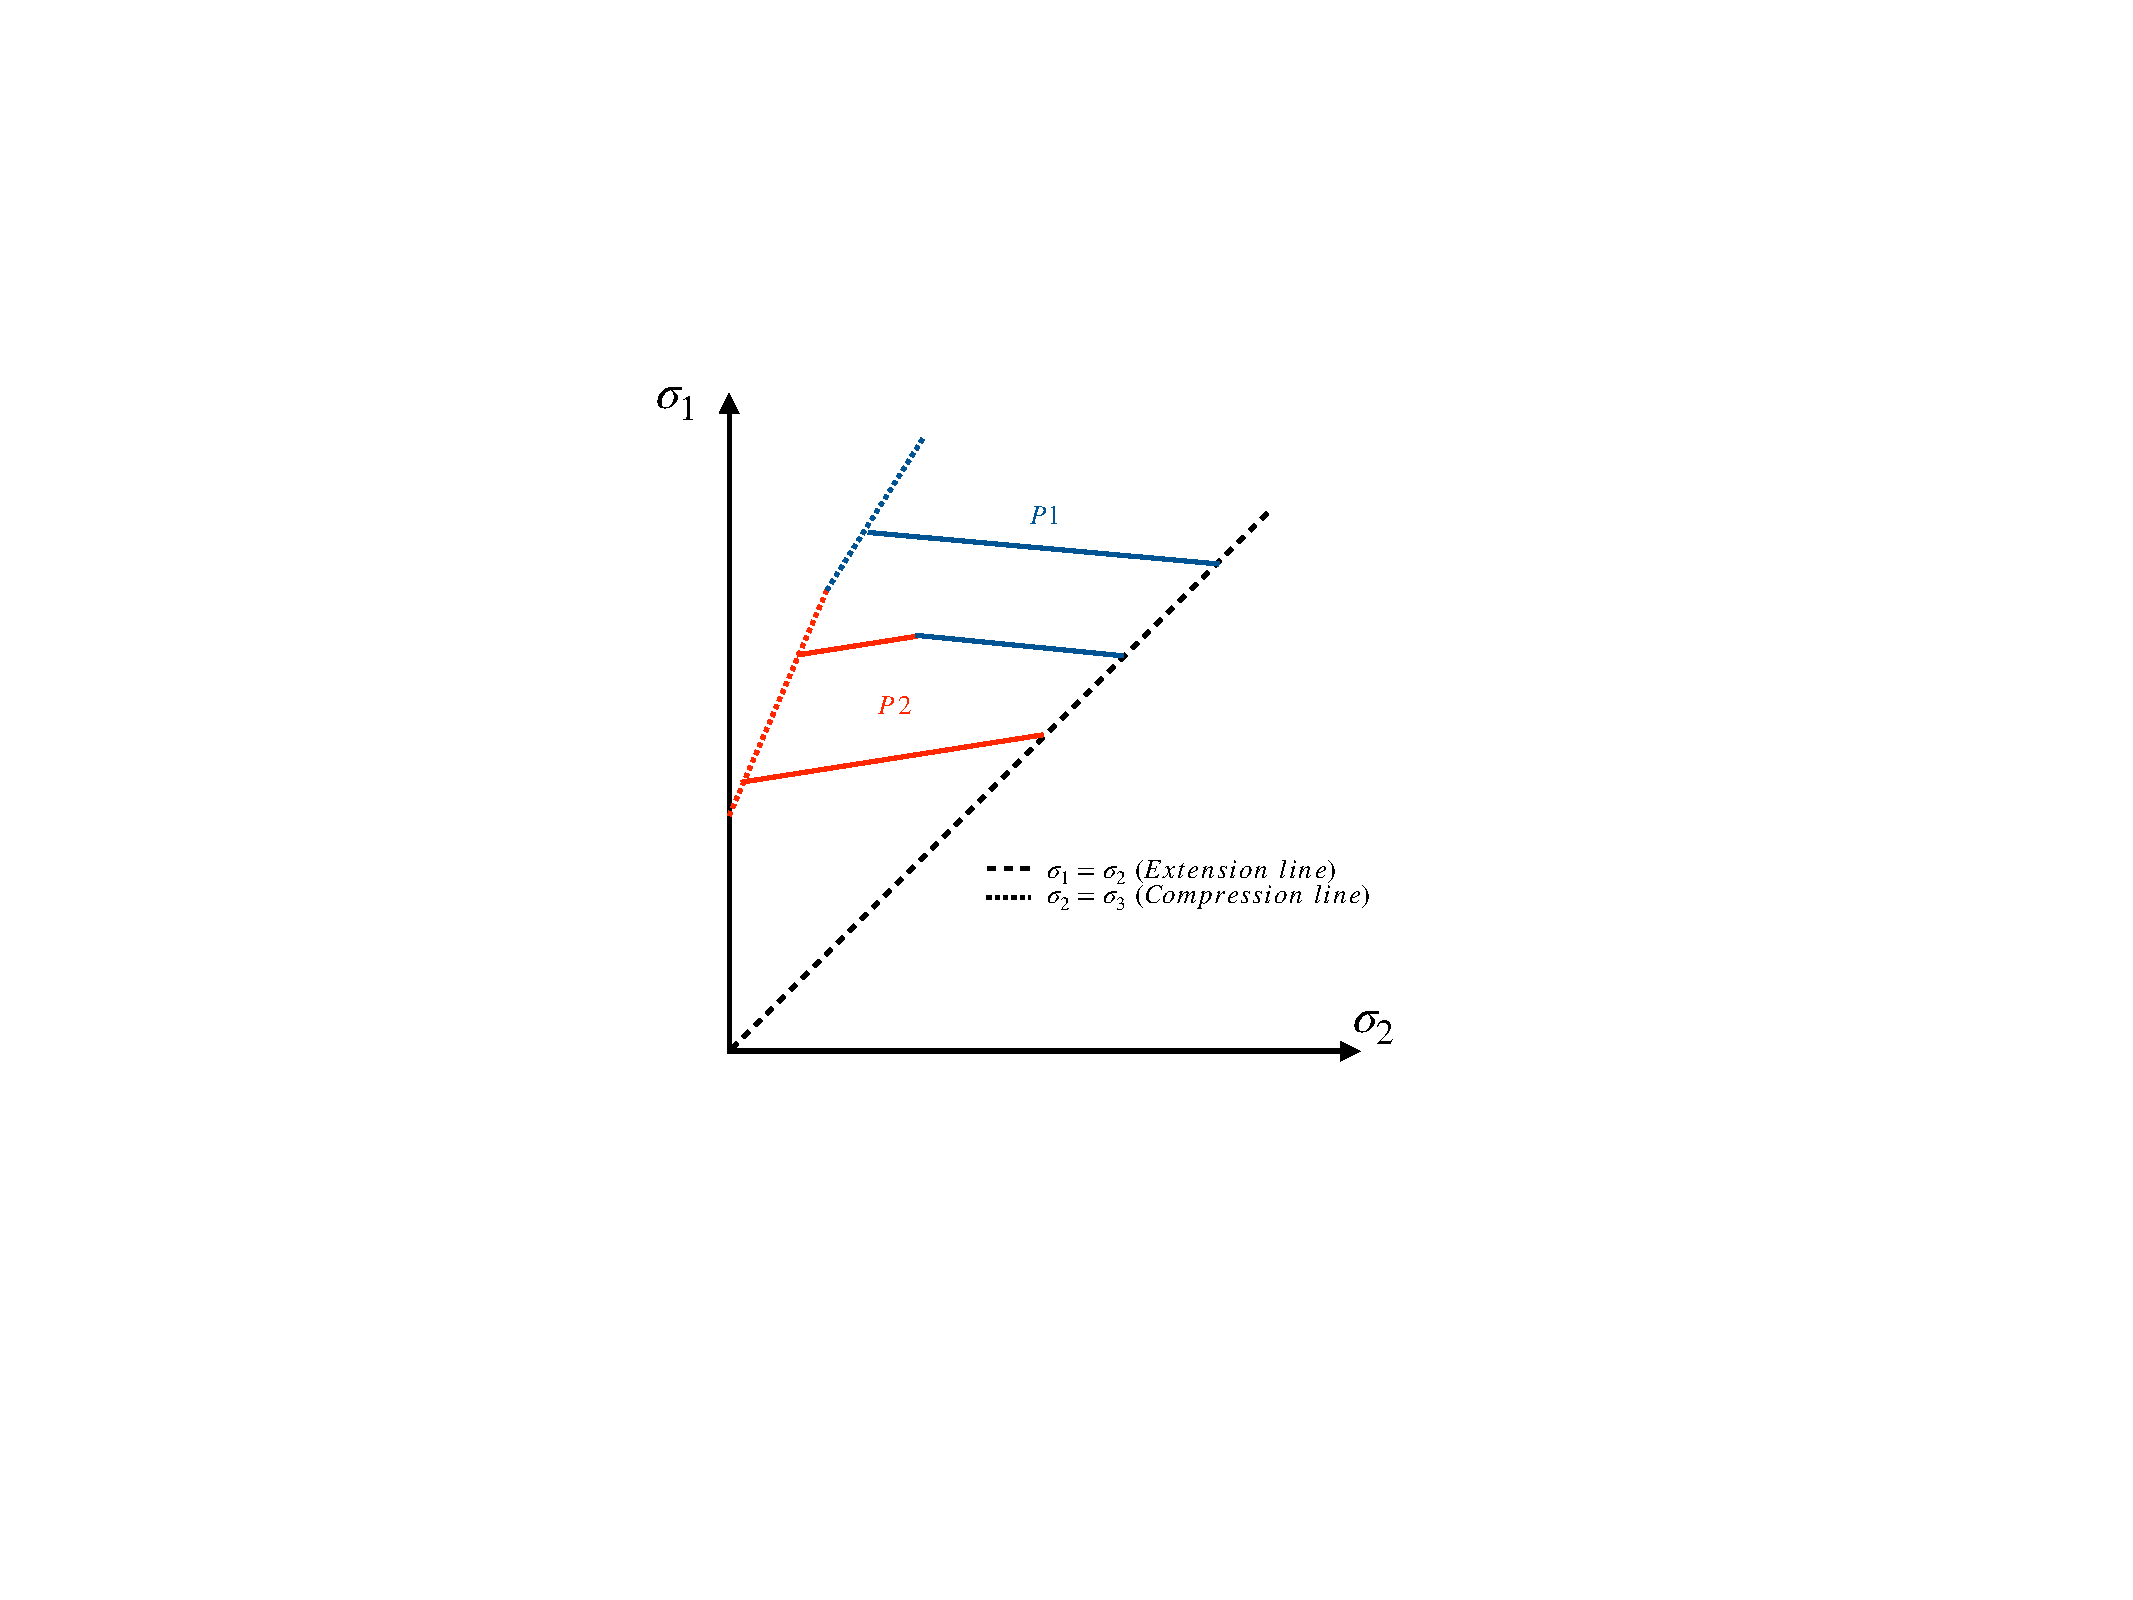
\includegraphics[width=0.6\columnwidth]{ch5/pmc6_sig2sig1_ske}
    \caption{Paul-Mohr-Coulomb 6-12-6 sided failure surface in $(\sigma_2-\sigma_1)$ plane}
    \label{fig5:6pmc_sig2sig1}
\end{figure}

%%%%%%%%%%%%%%%%%%%%%%%%%%%%%%%%%%%%%%%%%%%%%%%%%%%%%%%%%%%%%%%%%%%%%%%%%%%%%%%%%%
\subsection{Bi-linear fitting program}\label{ch5:algo}

The fitting of a six-parameters Paul-Mohr-Coulomb failure surface requires to create two datasets from the initial database of experiments results, one for each plane. Once defined, these datasets are used for planes fitting, following the procedure presented in Section \ref{ch2:pmcfit}. This repartition of the data points into different planes is a challenging step of the failure criterion fitting, as it should give the optimal solution for the database considered. 

One of this study objective was to create a program that automatically allocates data points to one of both planes, with the aim of getting a distribution that provide the best fitting for Paul-Mohr-Coulomb criterion. Moreover, it was crucial that this program was develop not only for the rock tested in this study (i.e. Dunnville Sandstone), but for any rock with available experimental data. 

This problem can be summarize by the following question:
\begin{center}
    \emph{How to automatize the allocation of data point into $P1$ or $P2$ in order to provide the most accurate fitting of Paul-Mohr-Coulomb criterion ?}
\end{center}
In the following paragraphs, the algorithm created to solve this problem will be described.

\subsubsection{Algorithm construction}

The algorithm developed to solve the problem presented above belongs to the \emph{Brute-force} algorithm family. This category is based on the following principal: every possibility offered by the database is tried and the one that gives the best solution to the problem is selected. The amount of data available in the case of rock testing ($n_{max}\sim 50$) is small enough to use this type of algorithm without having issues related to too high complexity. 

In the case of this study, the algorithm will test all the possible variations of data allocations to the $P1$ or $P2$ datasets which can be created form the rock database. For each possible combination, planes $P1$ and $P2$ are created by the computation of their coefficient and fitting parameters defined for Paul-Mohr-Coulomb, following the procedure presented in \ref{ch2:pmcfit}. Then, the Mean Square Error ($MSE$) is computed for each combination of datasets. Finally the data allocation variation that provides the minimal $MSE$ is selected as the solution of the two planes fitting problem.  

The algorithm proposed in this study can be apply to any rock testing database that contains results of the three principal stresses and the three invariants at failure (cf. Table \ref{tb5:database}). Indeed, the rock database is the only input that is required to run this algorithm. 

\subsubsection{Computation of the mean square error}

The error used in the computation of $MSE$ is equal to the distance of a data point, defined by $\sigma_I$, $\sigma_{II}$ and $\sigma_{III}$, from its belonging plane, defined by Equation \ref{eq2:PMC}:
\begin{equation}\label{eq5:error}
    err_{i} = A^{(j)}\sigma_I^{i}+B^{(j)}\sigma_{II}^{i}+C^{(j)}\sigma_{III}^{i} - 1
\end{equation}
where $i$ is the index of the data point in the database and $j$ indicates the plane number in which the data is allocated (i.e. $j=1$ for $P1$ and $j=2$ for $P2$). The Mean Square Error of a certain dataset combination $k$ is then computed as follow:
\begin{equation}\label{eq5:MSE}
    MSE_k = \frac{1}{n}\sum_{i=1}^{n} err_i^2
\end{equation}
The dataset combination $k$ that obtains the minimal $MSE$ value provides the best fitting solution for Paul-Mohr-Coulomb failure surface for the considered rock. 

\subsubsection{Program resources}

This algorithm was implemented in the programming language Python. The resources on the program developed to solve the two planes fitting problem are gathered in APPENDIX B. It contains the Python files required to run the program and a \emph{README} document that explains how to use the program. Moreover, all the code files are commented in detail to ease their use and understanding.  

%%%%%%%%%%%%%%%%%%%%%%%%%%%%%%%%%%%%%%%%%%%%%%%%%%%%%%%%%%%%%%%%%%%%%%%%%%%%%%%%%
\subsection{Dunnville Sandstone}

The program presented in the previous section was applied to the experimental results database of Dunnville Sandstone (cf. Table \ref{tb5:database}). The six parameters Paul-Mohr-Coulomb failure surface obtained is presented in the following paragraphs through its representation in the $(p-q)$, $(\sigma_2-\sigma_1)$, $\pi$- planes and in the principal stresses three-dimensional space. 

\subsubsection{Strength parameters computation}

The solution obtained from the least-square solution fitting describe in Chapter 2 (cf. Section \ref{ch2:pmcfit}, Equations \ref{eq2:PMCfinalform} and \ref{eq2:pmc_be}) is presented in Table \ref{tb5:dunn_sol1}. 

\begin{table} [p]
    \centering 
    \begin{tabular}{ccccc}
        \hline 
        Plane & $x_1^{(i)}$ & $x_2^{(i)}$ & $x_3^{(i)}$ \\
        \hline
        \hline
        $P1$ & 0.54 & -1.02 & 47.08 \\
        $P2$ & 1.39 & -1.10 & 15.47 \\
        \hline
    \end{tabular}
    \captionsetup{justification=centering}
    \caption{$P1$ and $P2$ least-square solutions $x$ for Dunnville sandstone}
    \label{tb5:dunn_sol1}
\end{table}

The strength parameters for Paul-Mohr-Coulomb failure criteria could be computed from Equations \ref{eq2:pmc_vo} to \ref{eq2:pmc_c}. The values obtained are gathered in Table \ref{tb5:dunn_strpara}. 

\begin{table} [p]
    \centering 
    \begin{tabular}{cccccc}
        \hline 
        Plane & $b_c^{(i)}$ [\si{MPa}] & $b_e^{(i)}$ [\si{MPa}] & $V_0^{(i)}$ [\si{MPa}] & $\phi_c^{(i)}$ [\si{\degree}] & $\phi_e^{(i)}$ [\si{\degree}] \\
        \hline
        \hline
        $P1$ & 47.1 & 34.1 & $86.9$ & $14.4$ & $12.1$\\
        $P2$ & 15.5 & 10.7 & $11.1$ & $34.3$ & $34.8$ \\
        \hline
    \end{tabular}
    \captionsetup{justification=centering}
    \caption{$P1$ and $P2$ strength parameters for Dunnville sandstone}
    \label{tb5:dunn_strpara}
\end{table}

\subsubsection{Graphical representation of the failure surface}

Knowing the strength parameters, the Paul-Mohr-Coulomb failure surface could be plotted in the $(p-q)$ plane using Equations \ref{eq2:PMC_pq} to \ref{eq2:pmc_b_pq} applied to each plane. The values of parameters $m_{c,e}$ and $c_{c,e}$ are presented in Table \ref{tb5:dunn_pq_para} and the $(p-q)$ plane plot is shown in Figure \ref{fig5:pmc6p_pq}.

\begin{table} [p]
    \centering 
    \begin{tabular}{ccccc}
        \hline 
        Plane & $m_c^{(i)}$ [-] & $m_e^{(i)}$ [-] & $c_c^{(i)}$ [\si{MPa}] & $c_e^{(i)}$ [\si{MPa}] \\
        \hline
        \hline
        $P1$ & 0.54 & 0.39 & 22.3 & 16.2 \\
        $P2$ & 1.39 & 0.96 & 7.61 & 5.26\\
        \hline
    \end{tabular}
    \captionsetup{justification=centering}
    \caption{$P1$ and $P2$ fitting parameters for Dunnville sandstone}
    \label{tb5:dunn_pq_para}
\end{table}

\begin{table} [p]
    \centering 
    \begin{tabular}{ccccc}
        \hline 
        Plane & $A^{(i)}$ & $B^{(i)}$ & $B^{(i)}$ \\
        \hline
        \hline
        $P1$ & \num{1.74d-2} & \num{4.26d-3} & \num{-3.32d-2} \\
        $P2$ & \num{3.47d-2} & \num{-8.31d-4} & \num{-1.24d-1} \\
        \hline
    \end{tabular}
    \captionsetup{justification=centering}
    \caption{Paul-Mohr-Coulomb general equation coefficients for Dunnville sandstone}
    \label{tb5:dunn_abc}
\end{table}

\begin{table} [p]
    \centering 
    \begin{tabular}{cccccc}
        \hline 
        Plane & $V_0^{(i)}$ [\si{MPa}] & $\phi_c^{(i)}$ [\si{\degree}] & $\phi_e^{(i)}$ [\si{\degree}] & $\bar{S}$ [\si{MPa}]\\
        \hline
        \hline
        $P1$ & $86.9$ & $14.4$ & $12.1$ & 9.12\\
        $P2$ & $11.1$ & $34.3$ & $34.8$ & 4.92\\
        \hline
    \end{tabular}
    \captionsetup{justification=centering}
    \caption{$P1$ and $P2$ strength parameters for Dunnville sandstone}
    \label{tb5:dunn_summary}
\end{table}

\begin{figure} [p]
    \centering
    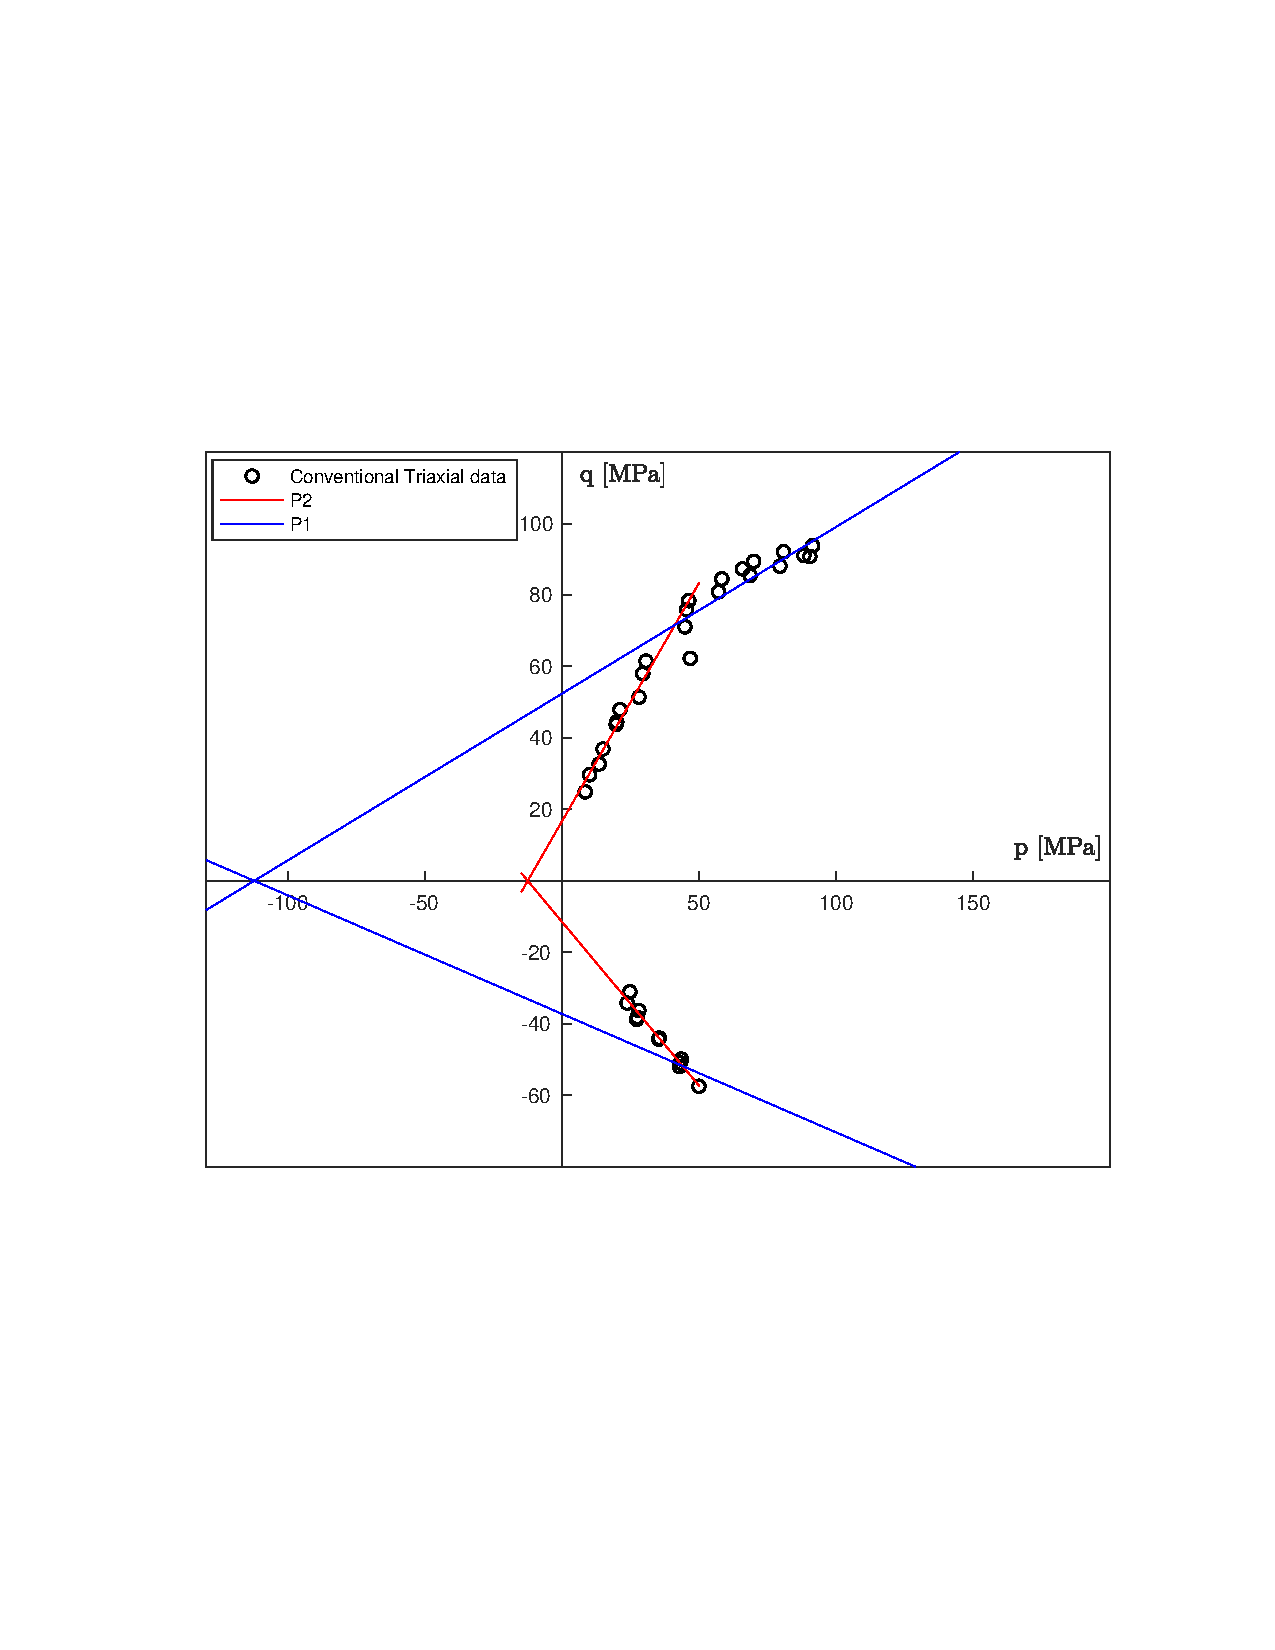
\includegraphics[width=0.8\columnwidth]{ch5/pmc6p_pq}
    \caption{Paul-Mohr-Coulomb failure surface in the $(p-q)$ plane for Dunnville Sandstone}
    \label{fig5:pmc6p_pq}
\end{figure}

The failure surface can also be plotted in the $(\sigma_2-\sigma_1)$ plane. Equation \ref{eq5:pmc_sig2sig1} provides the planes equation in this coordinates system using the general expression of the Paul-Mohr-Coulomb criterion, which coefficients $A$, $B$ and $C$ are presented in Table \ref{tb5:dunn_abc}. Figure \ref{fig5:pmc6p_sig1sig2} presents the six parameters failure surface for Dunnville Sandstone in the  $(\sigma_2-\sigma_1)$ plane.

\begin{figure} [p]
    \centering
    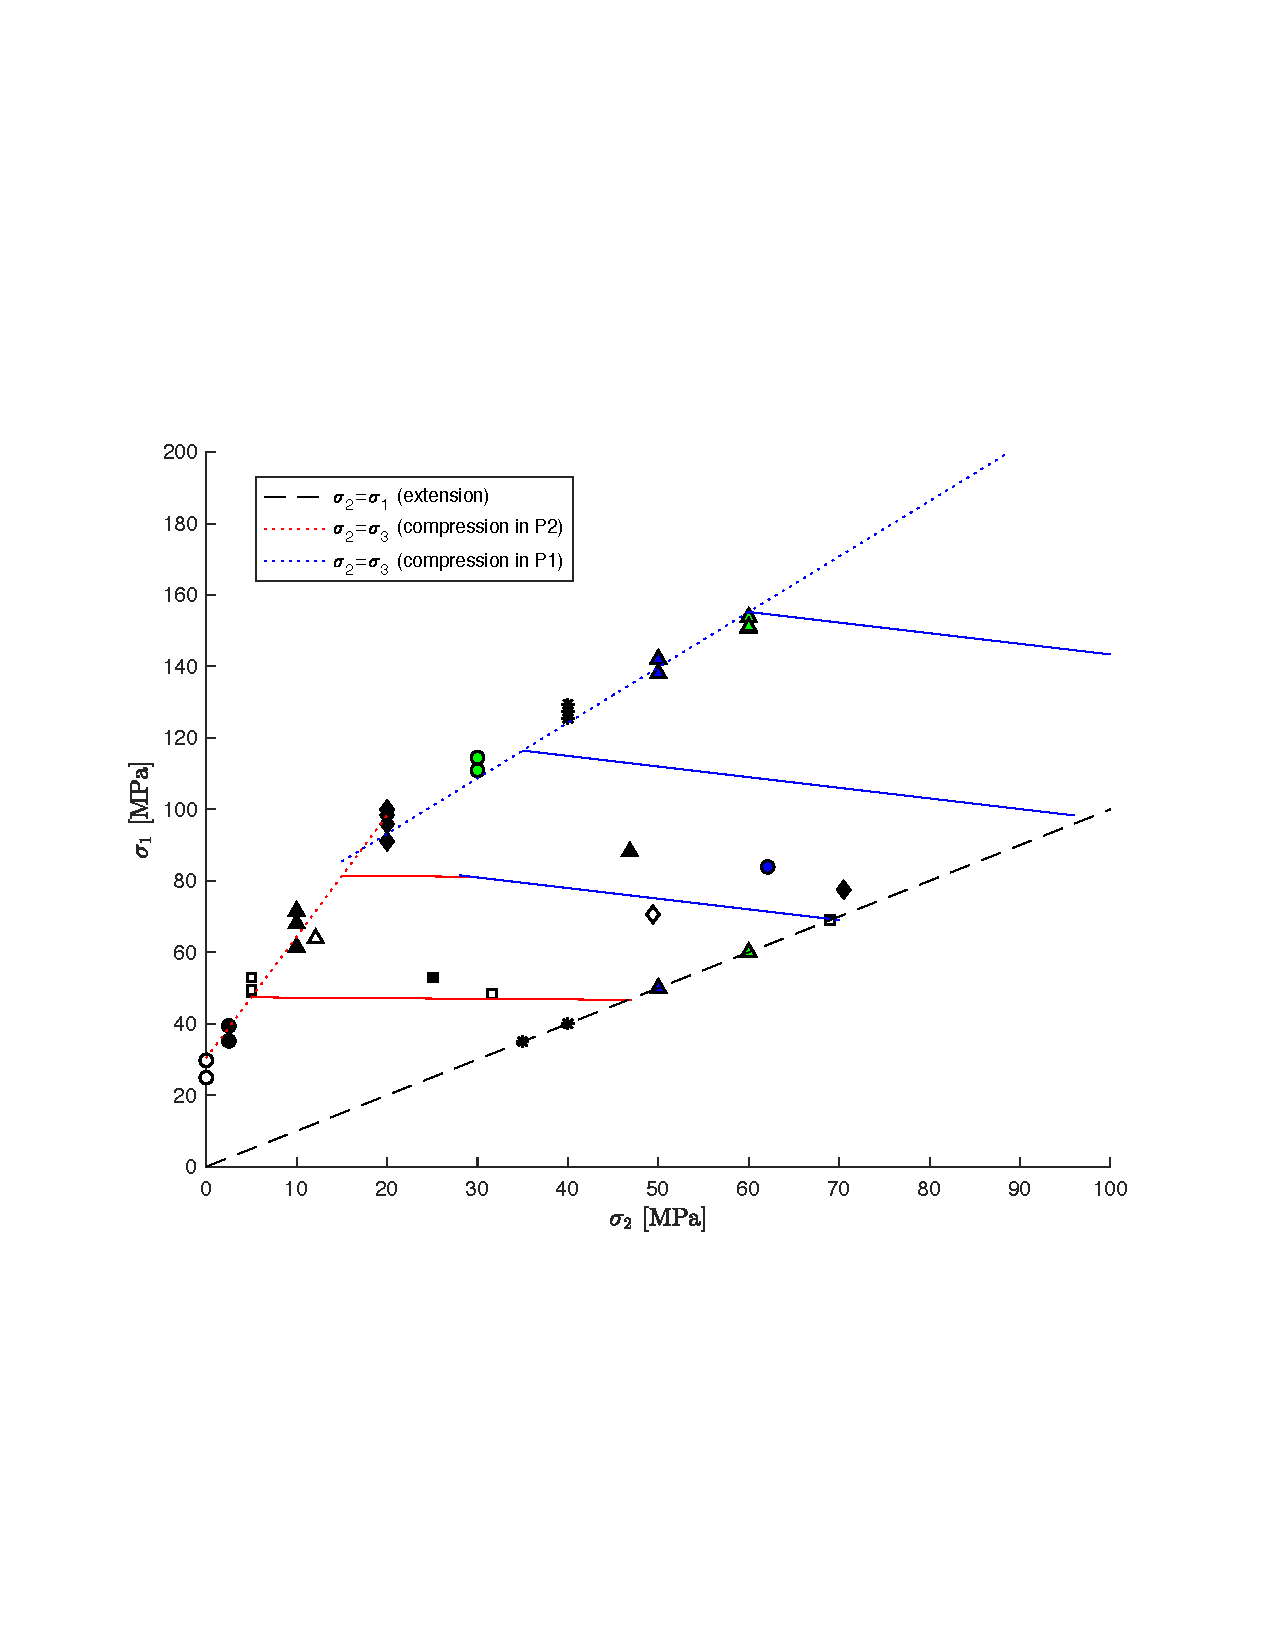
\includegraphics[width=0.8\columnwidth]{ch5/pmc6p_sig1sig2}
    \caption{Paul-Mohr-Coulomb failure surface in the $(\sigma_2-\sigma_1)$ plane for Dunnville Sandstone}
    \label{fig5:pmc6p_sig1sig2}
\end{figure}

The failure surface planes are also presented in the $\pi$-plane, obtained following the procedure described in Section \ref{ch2:PMC}. Figure \ref{fig5:pmc6p_pi_plane} shows the failure criterion in the $\pi$-plane at different mean stresses $p$ that correspond to true-triaxial experiments mean stresses at failure (i.e. $0^\circ < \theta < 60^\circ$ in Table \ref{tb5:database}). In addition, Figure \ref{fig5:pmc6p_pi_transi} presents the projection of the $P2$,$P2-P1$ transition and $P1$ pyramids on the $\pi$-plane. 

\begin{figure} [p]
    \centering
    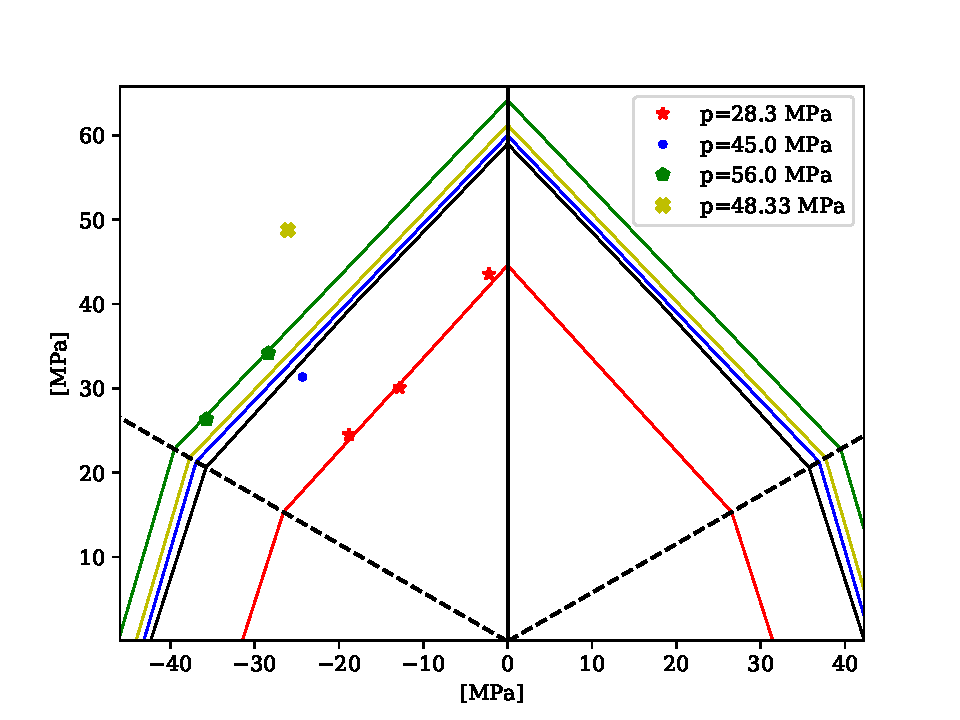
\includegraphics[width=0.9\columnwidth]{ch5/pmc6p_pi_pts2}
    \caption{Paul-Mohr-Coulomb failure surface in the $\pi$-plane for Dunnville Sandstone}
    \label{fig5:pmc6p_pi_plane}
\end{figure}
\begin{figure} [p]
    \centering
    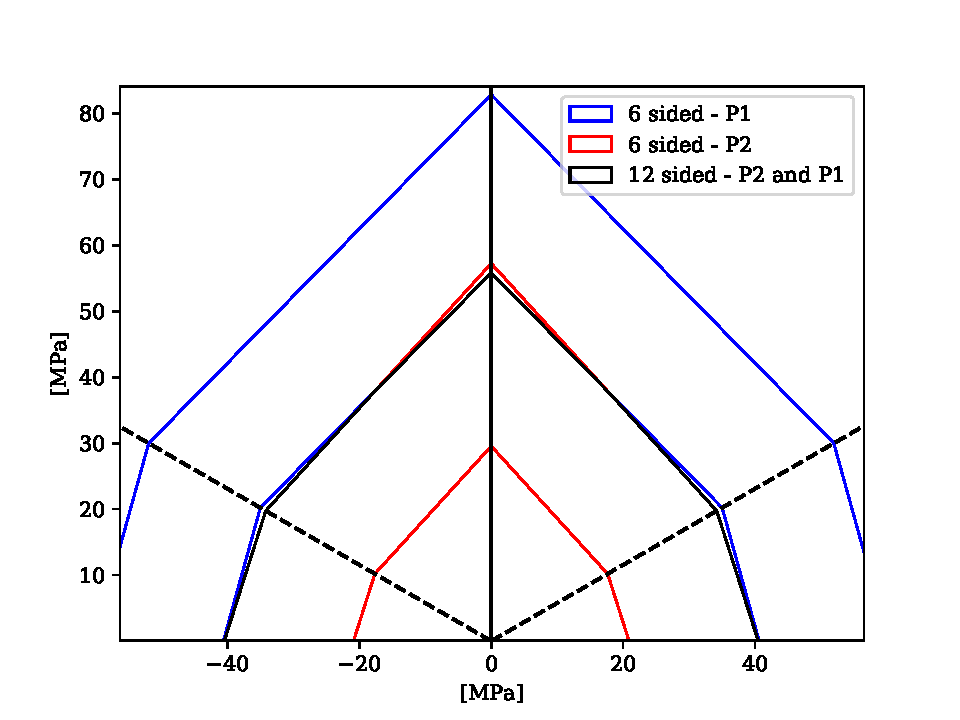
\includegraphics[width=0.9\columnwidth]{ch5/pmc6p_pi_transi2}
    \caption{6-12-6 sided pyramid projection in the $\pi$-plane for Dunnville Sandstone}
    \label{fig5:pmc6p_pi_transi}
\end{figure}

Finally, Figure \ref{fig5:pmc6p_3d} shows the 6-12-6 sided pyramid obtained for Dunnville Sandstone in the three-dimensional space. 

\begin{figure}
    \centering
    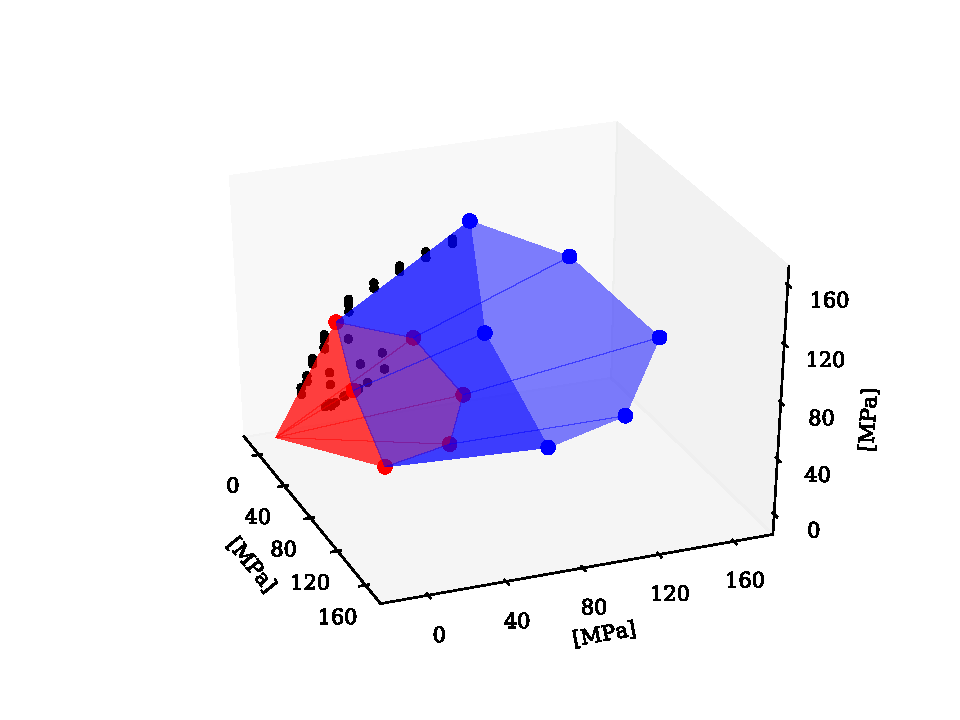
\includegraphics[width=\columnwidth]{ch5/pmc6p_3d1}
    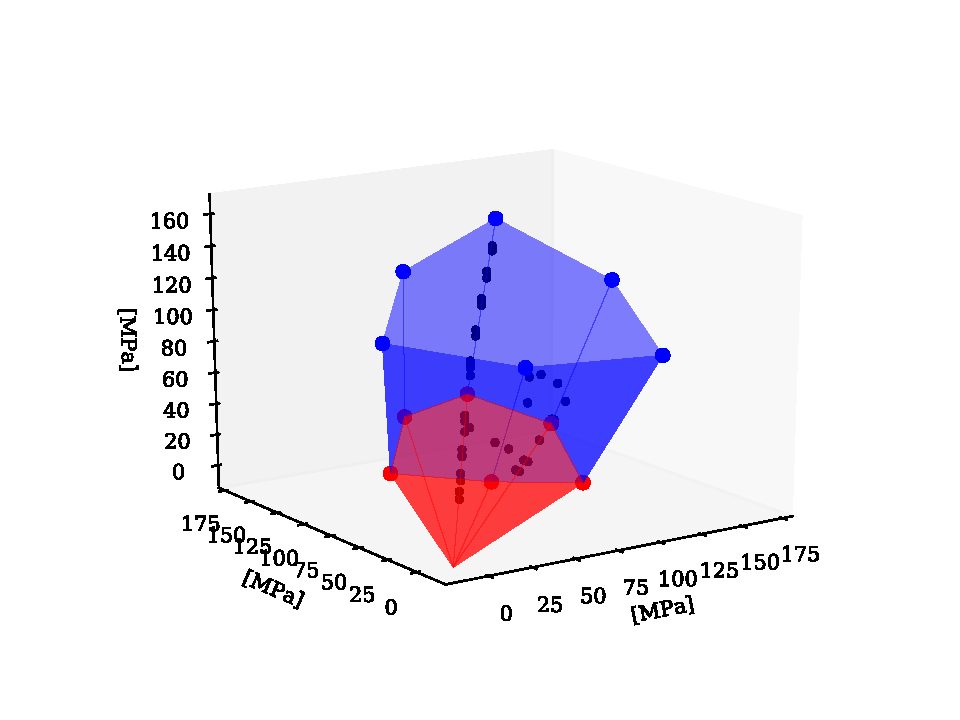
\includegraphics[width=\columnwidth]{ch5/pmc6p_3d2}
    \caption{Paul-Mohr-Coulomb 6-12-6 sided failure surface pyramid for Dunnville Sandstone}
    \label{fig5:pmc6p_3d}
\end{figure}

A summary of the Paul-Mohr-Coulomb six parameters solution and the mean standard deviation misfits obtained for Dunnville Sandstone is presented in Table \ref{tb5:dunn_summary}. The fittings provided by Mohr-Coulomb, Hoek-Brown, three and six parameters Paul-Mohr-Coulomb criteria can now be compared using the mean standard deviation misfits values obtained (cf. Table \ref{tb5:stand_dev}). 
The six parameters Paul-Mohr-Coulomb criterion provides the best prediction with the least mean standard deviation misfits for the two planes. This can be explained by the combination of the intermediate stress inclusion in the failure criterion general equation and the approximation of the failure surface non linearity, giving the most accurate states of stress prediction at failure. The observation of the six parameters Paul-Mohr-Coulomb and Hoek-Brown fittings in the $(p-q)$ and $\pi$- planes also presents for the first one a better approximation of the true-triaxial data points, but also of the axisymmetric ones, which wasn't the case with the three parameters Paul-Mohr-Coulomb. 

The program developed for the Paul-Mohr-Coulomb criterion was generalized so that it can be used to fit of other rocks. A summary of the results obtained for rocks with available database from literature is provided in APPENDIX D REF{APPENDIX D}.

%%%%%%%%%%%%%%%%%%%%%%%%%%%%%%%%%%%%%%%%%%%%%%%%%%%%%%%%%%%%%%%%%%%%%%%%%%%%%%%%%%%%%%%%%%%%%%%%%%%%%%%%%%%%%%%%%%%%%%%%%%%%%%%%%%%%%%%%%%%
\section{Discussion}

In this section, some remarks and comments are made on the work presented in this study. 

The previous sections provide a comparison of the four failure criteria principally based on the computation of the mean standard deviation misfits $\bar{S}$. This quantitive comparison indicator is based on the computation of the error between the predicted and real values of the major stress, and report the precision of the prediction provided by a failure criterion. Another comparison could also be relative to the failure surface. Indeed, a rigorous evaluation  of a failure criterion can be made by the computation of the distance between a data point and the failure surface. This type of error computation was used in this work in the \emph{Brute-force} algorithm developed for the six parameters Paul-Mohr-Coulomb fitting (cf. Section \ref{ch5:algo}). In this case, as well as for Mohr-Coulomb, the computation of the "point-plane" distance is made possible and convenient thanks to the explicit general equation of the planes that forms the failure surface. However, in the case of Hoek-Brown and other criteria defined by implicit equations, it becomes challenging to go through the mathematical derivations required to compute this distance. An interesting addition to this work would be to look at all the criteria evaluated here from the point of view of the "data-failure surface" distance, and to compare the quantitative indicators of the their accuracy.

The comparison of the three failure criteria revealed the importance of taking into account the intermediate stress in their formulation. First, the evaluation of the Mohr-Coulomb and Paul-Mohr-Coulomb indicates that even with the use of a linear criterion to approximate a non-linear failure surface, the one defined by a general equation in terms of the three principal stresses gives a better approximation of the data points. Moreover, the comparison between the Hoek-Brown and Paul-Mohr-Coulomb fittings reveals that a linear criterion that takes into account $\sigma_{II}$ gives a better fitting of the data from true triaxial experiments, which state of stress is more representative of what undergoes the rock in-situ. 

The work presented in this study showed that the six parameters Paul-Mohr-Coulomb failure criterion provides an accurate approximation of the failure surface as well as a good prediction of the state of stress at failure compared to popular criteria as Mohr-Coulomb and Hoek-Brown. Nonetheless, one criticism can be addressed to this criterion regarding the amount of experiments required to construct the bi-linear failure surface. Indeed, in order to built the failure surface of the three parameters Paul-Mohr-Coulomb criterion, three data points are needed, leading to a requirement of six points for the six parameters criterion. These six data points corresponds to the same number of experiments, ideally of different procedures, that is needed to be performed on the same rock. By carrying out this study in an very well equipped research environment, it was possible to perform multiple experiments under different conditions. However, this is hardly the case in the majority of rock mechanics and geo-engineering applications for which that amount of data is not always available. From this point of view, Mohr-Coulomb and Hoek-brown are more convenient to apply to a small amount of data, which is why they are popular and widely use. 

On the $\pi$-plane representations of the failure criteria (cf. Figure \ref{fig5:pmc6p_pi_plane}) the data point of the true triaxial experiment under plane strain condition (i.e. $p = 48.3$ \si{MPa}) presents an eccentricity from the failure surface but also from the "alignment" or "group" of other true-triaxial data (mainly performed under constant mean stress). Two possible explanation are proposed here. One can be that a mistake was made either during the experiment or in the analysis of its results. The second notices the possibility that the failure surface underestimate data from this type of experiments. Both highlight the need of an more detailed investigation on true triaxial experiments performed under various state of stress. However, it should be noted that preforming true triaxial experiments is challenging and time consuming, which makes difficult to gather data for the same rock.

Finally, a general comment can be made on the use of failure criteria. The not successful attempts made at performing a true triaxial experiment under constant mean stress pointed out the importance of failure stress state prediction. Indeed, the state of stress at failure should have been checked before running the test, revealing foreseen values of $\sigma_I$ and $\sigma_{II}$ to be reached, too close to failure of the specimen. Prediction of rock failure is crucial in geo-engineering applications, and research work should continue to seek for the best general failure criteria. 
